\documentclass{tufte-handout}\usepackage[]{graphicx}\usepackage[]{color}
%% maxwidth is the original width if it is less than linewidth
%% otherwise use linewidth (to make sure the graphics do not exceed the margin)
\makeatletter
\def\maxwidth{ %
  \ifdim\Gin@nat@width>\linewidth
    \linewidth
  \else
    \Gin@nat@width
  \fi
}
\makeatother

\definecolor{fgcolor}{rgb}{0.345, 0.345, 0.345}
\newcommand{\hlnum}[1]{\textcolor[rgb]{0.686,0.059,0.569}{#1}}%
\newcommand{\hlstr}[1]{\textcolor[rgb]{0.192,0.494,0.8}{#1}}%
\newcommand{\hlcom}[1]{\textcolor[rgb]{0.678,0.584,0.686}{\textit{#1}}}%
\newcommand{\hlopt}[1]{\textcolor[rgb]{0,0,0}{#1}}%
\newcommand{\hlstd}[1]{\textcolor[rgb]{0.345,0.345,0.345}{#1}}%
\newcommand{\hlkwa}[1]{\textcolor[rgb]{0.161,0.373,0.58}{\textbf{#1}}}%
\newcommand{\hlkwb}[1]{\textcolor[rgb]{0.69,0.353,0.396}{#1}}%
\newcommand{\hlkwc}[1]{\textcolor[rgb]{0.333,0.667,0.333}{#1}}%
\newcommand{\hlkwd}[1]{\textcolor[rgb]{0.737,0.353,0.396}{\textbf{#1}}}%
\let\hlipl\hlkwb

\usepackage{framed}
\makeatletter
\newenvironment{kframe}{%
 \def\at@end@of@kframe{}%
 \ifinner\ifhmode%
  \def\at@end@of@kframe{\end{minipage}}%
  \begin{minipage}{\columnwidth}%
 \fi\fi%
 \def\FrameCommand##1{\hskip\@totalleftmargin \hskip-\fboxsep
 \colorbox{shadecolor}{##1}\hskip-\fboxsep
     % There is no \\@totalrightmargin, so:
     \hskip-\linewidth \hskip-\@totalleftmargin \hskip\columnwidth}%
 \MakeFramed {\advance\hsize-\width
   \@totalleftmargin\z@ \linewidth\hsize
   \@setminipage}}%
 {\par\unskip\endMakeFramed%
 \at@end@of@kframe}
\makeatother

\definecolor{shadecolor}{rgb}{.97, .97, .97}
\definecolor{messagecolor}{rgb}{0, 0, 0}
\definecolor{warningcolor}{rgb}{1, 0, 1}
\definecolor{errorcolor}{rgb}{1, 0, 0}
\newenvironment{knitrout}{}{} % an empty environment to be redefined in TeX

\usepackage{alltt}

%\geometry{showframe}% for debugging purposes -- displays the margins
\usepackage{verbatim}
\usepackage{amsmath}
%\usepackage{natbib}
%\bibfont{\small} % Doesn't see to work...

% Set up the images/graphics package
\usepackage{graphicx}
%\setkeys{Gin}{width=\linewidth,totalheight=\textheight,keepaspectratio}
% \graphicspath{{graphics/}}


\title{Confidence Intervals %\thanks{}
}
\author[Marc Los Huertos]{Marc Los Huertos}
%\date{}  % if the \date{} command is left out, the current date will be used


% \SweaveOpts{prefix.string=graphics/plot} % Created a "graphics" subdirectory to 

\setsidenotefont{\color{blue}}
% \setcaptionfont{hfont commandsi}
% \setmarginnotefont{\color{blue}}
% \setcitationfont{\color{gray}}

% The following package makes prettier tables.  We're all about the bling!
%\usepackage{booktabs}

% Small sections of multiple columns
%\usepackage{multicol}
\IfFileExists{upquote.sty}{\usepackage{upquote}}{}
\begin{document}

\maketitle% this prints the handout title, author, and date

\begin{abstract}
\noindent An important considerations with univariate data is the development of confidence intervals and forms the foundation for hypothesis testing. As you can probably guess, confidence intervals are based on the distribution of the data. Data with lots of variability will have wide confidence intervals, while data with low variability will have narrow confidence intervals. 

There are two main approaches in developing confidence intervals. One relies on the use of theoretical probability distributions. Another method uses the data themselves to create randomized sample subsets (bootstrapping) to create confidence intervals. We will learn several methods because each are used in environmental sciences to varying degrees. I have decribed the former in this handout, but may add bootstrapping soon. 
\end{abstract}

%\printclassoptions

% Setting up the margins, etc for R


\section{Why Confidence Intervals?}

Confidence intervals are used to indicate the reliability of an estimate. How likely the interval is to contain the parameter is determined by the confidence level. Increasing the desired confidence level will widen the confidence interval (see Figure~\ref{fig:3rule}). Based on a foundational understanding of confidence intervals allows us to extend our interpretations of the data toward a hypothesis testing perspective, which we'll get into more during the semester.

\section{Where are Confidence Intervals Used?}

Confidence intervals can be calculated for a range of statistics, including the mean, slope and intercept of a linear model, among other things. We'll concentrate on the what confidence intervals of the population and sample mean at this point, but keep in mind the concept can be applied to many parameter estimates.

\begin{marginfigure}
	\centering
		
\includegraphics[width=1.00\textwidth]{Investor_confidence500.jpg}
	\caption{Confidence abounds without bounds.}
	\label{fig:Investor_confidence500}
\end{marginfigure}

\section{Defining Some Terms}

\subsection{Populations and Samples}

In general, environmental scientists can't measure the entire population. For example, a complete audit of all the recycling would be impossible for our class!  Instead, we sample from the population. Statisticians have have developed semi-consistant symbology for various statistics based on populations and samples. 

A population mean for example is usually referred to by the Greek letter, $\mu$. While for a sample, the mean might be referred to as $\bar{y}$ (or $\bar{x}$). The spread of data, or variance, in a population is referred to as $\sigma^2$, again a Greek letter. The population variance is often referred to as $s^2$. In general, we don't know $\mu$ or $\sigma^2$, so we can estimate them and develop confidence intervals that probably include the true $\mu$. Notice the word, ''probably.''  In other words, we our intervals in terms of probabilities!\sidenote{When you hear the word probably, it might be useful to think about how this implies a probability distribution.}

\subsection{The difference between $\mu$ and $\bar{x}$}

To illustrate the difference, let's create a dataset of 1000 random numbers from a normal distribution with a mean of 10 and standard deviation of 1. We'll let this represent an entire population.\sidenote{I rounded the values to the nearest tenth, to keep the printouts more managable.} 
\begin{knitrout}
\definecolor{shadecolor}{rgb}{0.969, 0.969, 0.969}\color{fgcolor}\begin{kframe}
\begin{alltt}
\hlkwd{set.seed}\hlstd{(}\hlnum{123}\hlstd{)}
\hlstd{N1000} \hlkwb{=} \hlkwd{round}\hlstd{(}\hlkwd{rnorm}\hlstd{(}\hlkwc{n}\hlstd{=} \hlnum{1000}\hlstd{,} \hlkwc{mean} \hlstd{=} \hlnum{10}\hlstd{,} \hlkwc{sd} \hlstd{=} \hlnum{1}\hlstd{),} \hlnum{1}\hlstd{)}
\end{alltt}
\end{kframe}
\end{knitrout}

The distribution of the data (Figure~\ref{fig:hist_pop}), resembles a normal distribution, which is reassuring since we created it using a random number generator that uses the normal probability distribution. 

\begin{marginfigure}
\begin{knitrout}
\definecolor{shadecolor}{rgb}{0.969, 0.969, 0.969}\color{fgcolor}
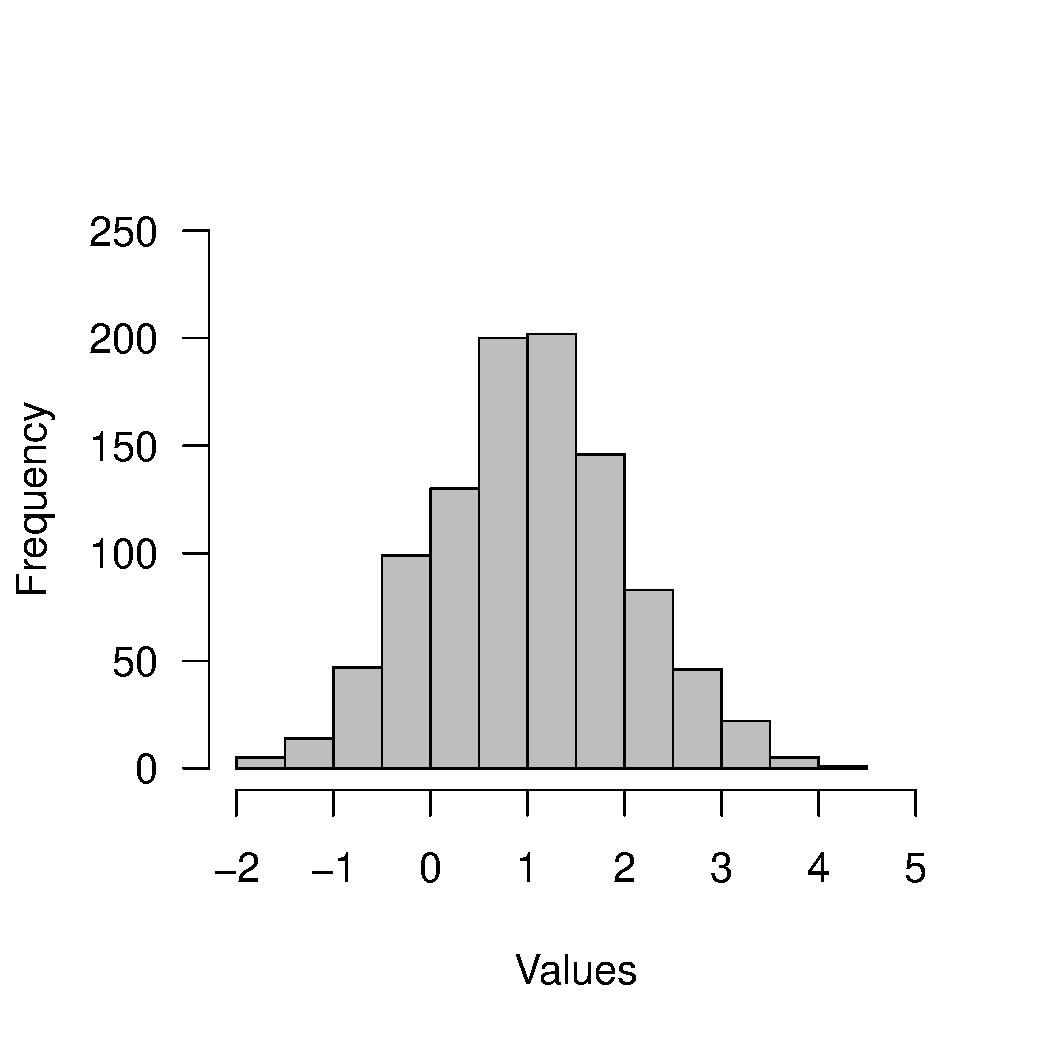
\includegraphics[width=\maxwidth]{figure/unnamed-chunk-3-1} 

\end{knitrout}
\caption{Frequency distribution of population.}
\label{fig:hist_pop}
\end{marginfigure}

These data will represent the population (N) and has a mean or $\mu$ of 10.02. The values range from 7.2 to 13.2 (Figure~\ref{fig:hist_pop}). From this dataset, we can create several dataset sets by random sampling the vector with different n (n = 100, n = 20, n = 10, n = 5). 

\begin{knitrout}
\definecolor{shadecolor}{rgb}{0.969, 0.969, 0.969}\color{fgcolor}\begin{kframe}
\begin{alltt}
\hlstd{n100} \hlkwb{=} \hlkwd{sample}\hlstd{(N1000,} \hlkwc{size} \hlstd{=} \hlnum{100}\hlstd{)}
\hlstd{n20} \hlkwb{=} \hlkwd{sample}\hlstd{(N1000,} \hlkwc{size} \hlstd{=} \hlnum{20}\hlstd{)}
\hlstd{n10} \hlkwb{=} \hlkwd{sample}\hlstd{(N1000,} \hlkwc{size} \hlstd{=} \hlnum{10}\hlstd{)}
\hlstd{n5} \hlkwb{=} \hlkwd{sample}\hlstd{(N1000,} \hlkwc{size} \hlstd{=} \hlnum{5}\hlstd{)}
\end{alltt}
\end{kframe}
\end{knitrout}

With a size or n of ten values from our population, I have obtained the following result: 
\begin{knitrout}
\definecolor{shadecolor}{rgb}{0.969, 0.969, 0.969}\color{fgcolor}\begin{kframe}
\begin{alltt}
\hlstd{n10}
\end{alltt}
\begin{verbatim}
##  [1] 10.2 11.4 10.1  9.3  9.8  9.4 10.6 11.0 10.4 10.0
\end{verbatim}
\end{kframe}
\end{knitrout}
\noindent and a mean or $\bar{y}$ = 10.22. These values certainly fall within the distribution of the population (Figure~\ref{fig:hist_pop}).

\subsection{R's Default Boxplot}

One of the confusing aspects when learning R and statistics at the same time is the range of subtle discrepencies between the vocabulary in statistics, parameter symbology, and how R implments statistics. But just as we learn a language we use content (e.g. literature), I have found it best to learn statistics while learning to use the R language. 

Nevertheless, the sublties land hard on us when we are just trying to keep up with the statistical concepts. The \texttt{boxplot} function in R is easy to make and provides a lot of information, but it's not always clear what is being displayed. For example, the \texttt{boxplot()} function displays the median (for our ten sample vector = 10.15 and not the mean (10.22). In Figure~\ref{fig:default_bp}A, the boxplot displays the median, interquarile range, and range. But in many cases, the sample might have some points that seem to be way outside the normal range. In those cases R creates a figure with a more complex set of rules. We won't go into these at this point, but not the differences between Figure~\ref{fig:default_bp}A and Figure~\ref{fig:default_bp}B. 

\begin{figure}
\caption{Boxplot where panel A displays the following information for our 10 sample vector: median =10.15; Range = 9.3, 11.4; and interquartile range = 9.85, 10.55. Panel B identifies an ``outlier" using obscure rules and changing the range to exclude the outlier. I included the value of 14.8 with the vector to demonstrate this change. Weird. Note: I rotated the y-axis labels to make it easier to read. I try to do this with all my figures to make it easier to read.}
\label{fig:default_bp}
\begin{knitrout}
\definecolor{shadecolor}{rgb}{0.969, 0.969, 0.969}\color{fgcolor}
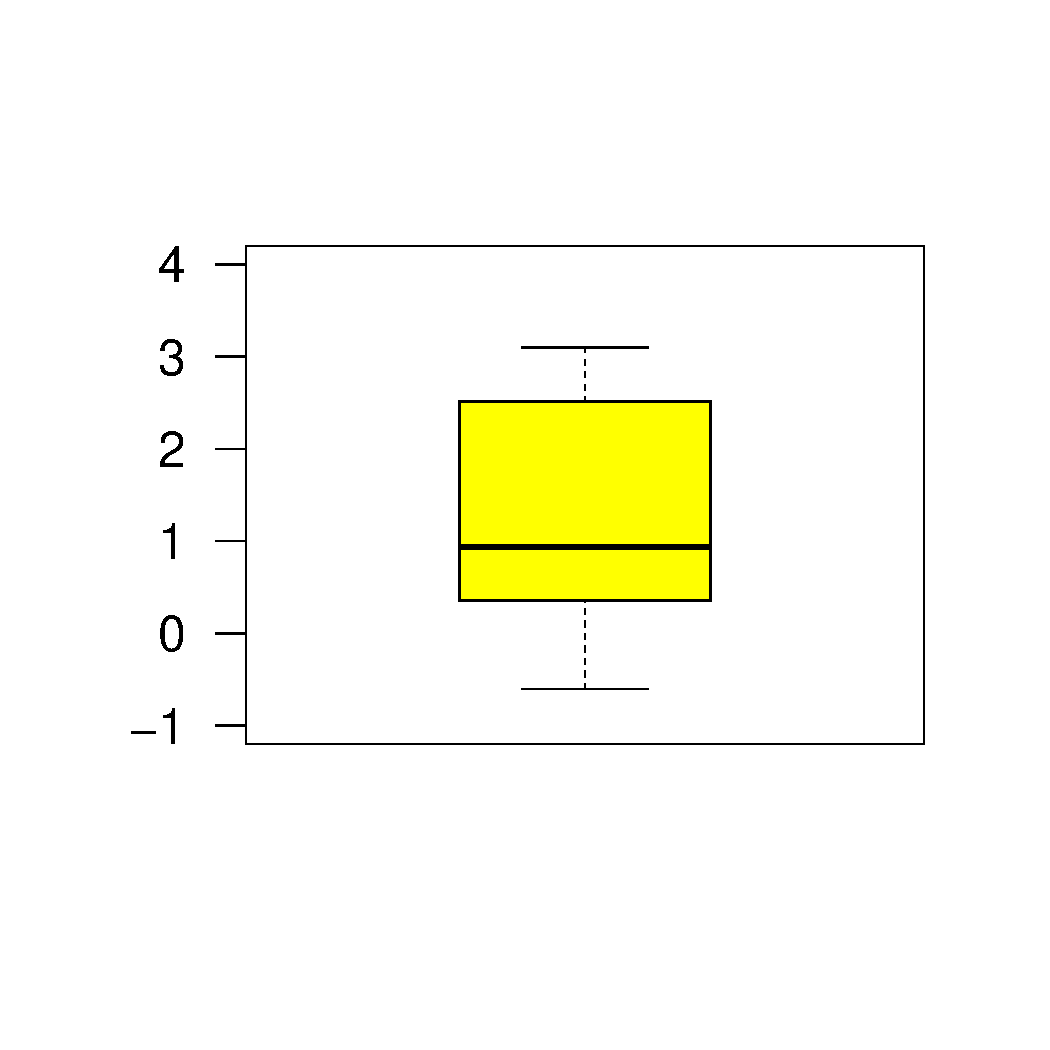
\includegraphics[width=\maxwidth]{figure/unnamed-chunk-6-1} 

\end{knitrout}
\end{figure}

%Let's see if we can label the graphic directly!
In the end, the \texttt{boxplot()} function is very useful to quickly summarize the data, but in most cases, we tend to describe the data using a more precise set of measures. The standard deviation is the most commonly used parameter to measure the variability or spread of the data. 

\subsection{Exploring the Waste Audit Data}

Let's `read' the data into r, with the \texttt{read.csv()} function.
\begin{knitrout}
\definecolor{shadecolor}{rgb}{0.969, 0.969, 0.969}\color{fgcolor}\begin{kframe}
\begin{alltt}
\hlstd{Unsorted.csv} \hlkwb{=} \hlstr{"/home/CAMPUS/mwl04747/github/beginnersluck/Confidence_Intervals/2019_EA30F_Waste_Audit_Unsorted.csv"}

\hlstd{Sorted.csv} \hlkwb{=} \hlstr{"/home/CAMPUS/mwl04747/github/beginnersluck/Confidence_Intervals/2019_EA30F_Waste_Audit_Sorted_v2.csv"}
\hlcom{# Read Raw Data}
\hlstd{Unsorted} \hlkwb{=} \hlkwd{read.csv}\hlstd{(Unsorted.csv)}
\hlstd{Sorted} \hlkwb{=} \hlkwd{read.csv}\hlstd{(Sorted.csv)}
\end{alltt}
\end{kframe}
\end{knitrout}

Now that we have imported the data into R, we will not process some of the data to prepare for the analysis. For example, let's caculate the percentage of sorted items, remove the plastic film category, and shorten the compostable name to simply compost. 

\begin{knitrout}
\definecolor{shadecolor}{rgb}{0.969, 0.969, 0.969}\color{fgcolor}\begin{kframe}
\begin{alltt}
\hlstd{Sorted}\hlopt{$}\hlstd{Percent} \hlkwb{=} \hlstd{(Sorted}\hlopt{$}\hlstd{NetMass}\hlopt{/}\hlstd{Sorted}\hlopt{$}\hlstd{Total)}\hlopt{*}\hlnum{100}
\hlstd{Sorted} \hlkwb{=} \hlkwd{subset}\hlstd{(Sorted,} \hlkwc{subset}\hlstd{=Type}\hlopt{!=}\hlstr{"Plastic Film"}\hlstd{)}
\hlkwd{levels}\hlstd{(Sorted}\hlopt{$}\hlstd{Type)[}\hlkwd{levels}\hlstd{(Sorted}\hlopt{$}\hlstd{Type)}\hlopt{==}\hlstr{"Compostable"}\hlstd{]} \hlkwb{<-} \hlstr{"Compost"}
\end{alltt}
\end{kframe}
\end{knitrout}

Be sure to check the results as you go and convince yourself how these work by looking online to see how these functions work. 

Anyone who has worked with quantitiative data knows that data entry errors can be a major headache if they are not caught early. Thus, we'll use a couple of methods to evaluate potential data entry errors. 

\begin{figure*}
\caption{Sorted Percent Mass from Recycling Bags}
\label{fig:percent_bp}
\begin{knitrout}
\definecolor{shadecolor}{rgb}{0.969, 0.969, 0.969}\color{fgcolor}
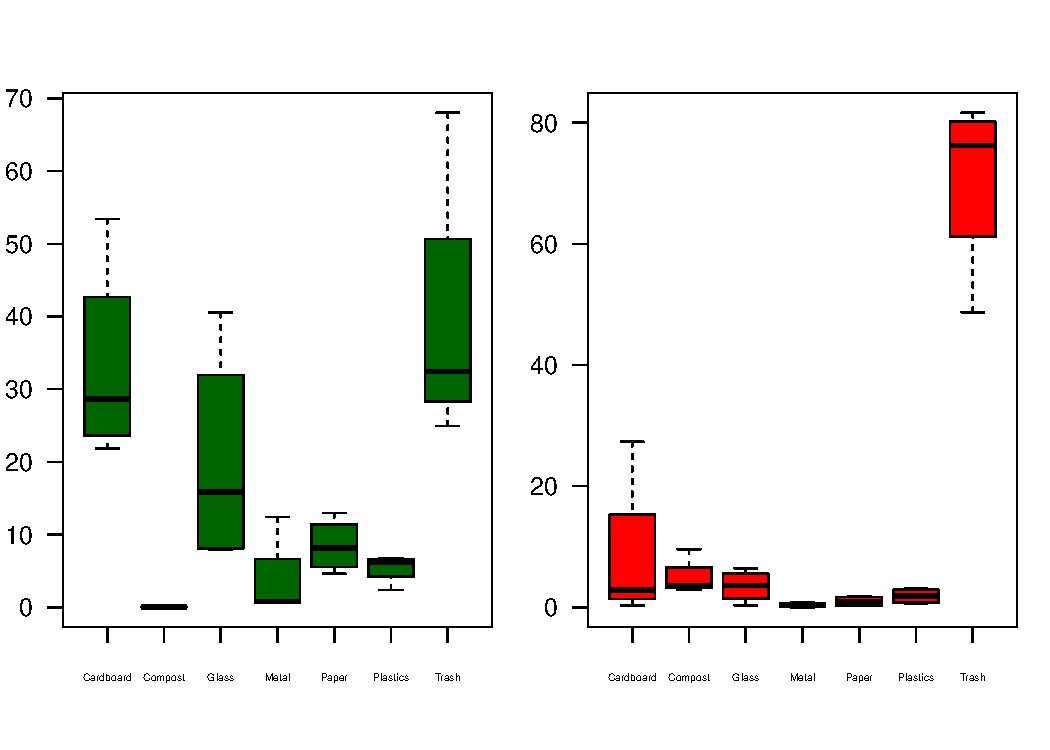
\includegraphics[width=\maxwidth]{figure/unnamed-chunk-9-1} 

\end{knitrout}
\end{figure*}

In the case of Figure~\ref{fig:percent_bp}, We can see that the trash is relatively high in both types of unsorted bags, e.g. there a fair amount trash in both the recyling and trash containers. But I wonder if the overlapping interval is statistically significant?  If they are the same, then the percentage of trash is being put in both containers without regard of the intended use. The boxplot is useful to start with, but we can't draw statistical conclusions on this yet.  

\subsection{Measuring the Spread}

We can calculate the variance of the sample using the following formula: 
\begin{equation}
s^2 = \frac{\sum(y_i - \bar{y})^2}{n-1}
\end{equation}

Let's apply this equation, so you can see how it works! First, we'll take the difference between a measurment and the mean.\sidenote{We will use the vector index to subset each variable -- see ``Blue Book'' for indexing if you want more information on this procedure.} Let's start with the first observation:
\begin{knitrout}
\definecolor{shadecolor}{rgb}{0.969, 0.969, 0.969}\color{fgcolor}\begin{kframe}
\begin{alltt}
\hlstd{n10[}\hlnum{1}\hlstd{]} \hlopt{-} \hlkwd{mean}\hlstd{(n10)}
\end{alltt}
\begin{verbatim}
## [1] -0.02
\end{verbatim}
\end{kframe}
\end{knitrout}

Next we square the difference\sidenote{R did scientific notation on this, I'll need to fix this in the near future.}
\begin{knitrout}
\definecolor{shadecolor}{rgb}{0.969, 0.969, 0.969}\color{fgcolor}\begin{kframe}
\begin{alltt}
\hlstd{(n10[}\hlnum{1}\hlstd{]} \hlopt{-} \hlkwd{mean}\hlstd{(n10))}\hlopt{^}\hlnum{2}
\end{alltt}
\begin{verbatim}
## [1] 4e-04
\end{verbatim}
\end{kframe}
\end{knitrout}
\noindent Now we'll do this for each of the remaining observations:
\begin{knitrout}
\definecolor{shadecolor}{rgb}{0.969, 0.969, 0.969}\color{fgcolor}\begin{kframe}
\begin{alltt}
\hlstd{(n10[}\hlnum{2}\hlstd{]} \hlopt{-} \hlkwd{mean}\hlstd{(n10))}\hlopt{^}\hlnum{2}
\end{alltt}
\begin{verbatim}
## [1] 1.3924
\end{verbatim}
\begin{alltt}
\hlstd{(n10[}\hlnum{3}\hlstd{]} \hlopt{-} \hlkwd{mean}\hlstd{(n10))}\hlopt{^}\hlnum{2}
\end{alltt}
\begin{verbatim}
## [1] 0.0144
\end{verbatim}
\begin{alltt}
\hlstd{(n10[}\hlnum{4}\hlstd{]} \hlopt{-} \hlkwd{mean}\hlstd{(n10))}\hlopt{^}\hlnum{2}
\end{alltt}
\begin{verbatim}
## [1] 0.8464
\end{verbatim}
\begin{alltt}
\hlstd{(n10[}\hlnum{4}\hlstd{]} \hlopt{-} \hlkwd{mean}\hlstd{(n10))}\hlopt{^}\hlnum{2}
\end{alltt}
\begin{verbatim}
## [1] 0.8464
\end{verbatim}
\end{kframe}
\end{knitrout}
These are ``deviates.'' Then we add the deviates together (which is what the $\Sigma$ symbol is tell us to do). We'll call the sum of squared deviates:

\begin{knitrout}
\definecolor{shadecolor}{rgb}{0.969, 0.969, 0.969}\color{fgcolor}\begin{kframe}
\begin{alltt}
\hlstd{(sum_of_squared_deviates} \hlkwb{=} \hlstd{(n10[}\hlnum{1}\hlstd{]} \hlopt{-} \hlkwd{mean}\hlstd{(n10))}\hlopt{^}\hlnum{2} \hlopt{+}
   \hlstd{(n10[}\hlnum{2}\hlstd{]} \hlopt{-} \hlkwd{mean}\hlstd{(n10))}\hlopt{^}\hlnum{2} \hlopt{+} \hlstd{(n10[}\hlnum{3}\hlstd{]} \hlopt{-} \hlkwd{mean}\hlstd{(n10))}\hlopt{^}\hlnum{2} \hlopt{+}
   \hlstd{(n10[}\hlnum{4}\hlstd{]} \hlopt{-} \hlkwd{mean}\hlstd{(n10))}\hlopt{^}\hlnum{2} \hlopt{+} \hlstd{(n10[}\hlnum{5}\hlstd{]} \hlopt{-} \hlkwd{mean}\hlstd{(n10))}\hlopt{^}\hlnum{2} \hlopt{+}
   \hlstd{(n10[}\hlnum{6}\hlstd{]} \hlopt{-} \hlkwd{mean}\hlstd{(n10))}\hlopt{^}\hlnum{2} \hlopt{+} \hlstd{(n10[}\hlnum{7}\hlstd{]} \hlopt{-} \hlkwd{mean}\hlstd{(n10))}\hlopt{^}\hlnum{2} \hlopt{+}
   \hlstd{(n10[}\hlnum{8}\hlstd{]} \hlopt{-} \hlkwd{mean}\hlstd{(n10))}\hlopt{^}\hlnum{2} \hlopt{+} \hlstd{(n10[}\hlnum{9}\hlstd{]} \hlopt{-} \hlkwd{mean}\hlstd{(n10))}\hlopt{^}\hlnum{2} \hlopt{+}
   \hlstd{(n10[}\hlnum{10}\hlstd{]} \hlopt{-} \hlkwd{mean}\hlstd{(n10))}\hlopt{^}\hlnum{2}\hlstd{)}
\end{alltt}
\begin{verbatim}
## [1] 3.936
\end{verbatim}
\end{kframe}
\end{knitrout}

We take the sum of these and divide by the degrees of freedom.\sidenote{Degree of freedom is extremely complicated to explain without tons of theory. For now, just rest assured that it works. If we have time, we'll delve into this more.}

\begin{knitrout}
\definecolor{shadecolor}{rgb}{0.969, 0.969, 0.969}\color{fgcolor}\begin{kframe}
\begin{alltt}
\hlstd{sum_of_squared_deviates}\hlopt{/}\hlstd{(}\hlnum{10}\hlopt{-}\hlnum{1}\hlstd{)}
\end{alltt}
\begin{verbatim}
## [1] 0.4373333
\end{verbatim}
\begin{alltt}
\hlkwd{sqrt}\hlstd{(sum_of_squared_deviates}\hlopt{/}\hlstd{(}\hlnum{10}\hlopt{-}\hlnum{1}\hlstd{))}
\end{alltt}
\begin{verbatim}
## [1] 0.6613118
\end{verbatim}
\end{kframe}
\end{knitrout}
\noindent Thankfully, we don't need to use all of this tedious code to generate the variance and standard deviation. We can use \texttt{var()} and \texttt{sd()}. 
\begin{knitrout}
\definecolor{shadecolor}{rgb}{0.969, 0.969, 0.969}\color{fgcolor}\begin{kframe}
\begin{alltt}
\hlkwd{var}\hlstd{(n10)}
\end{alltt}
\begin{verbatim}
## [1] 0.4373333
\end{verbatim}
\begin{alltt}
\hlkwd{sd}\hlstd{(n10)}
\end{alltt}
\begin{verbatim}
## [1] 0.6613118
\end{verbatim}
\end{kframe}
\end{knitrout}

\noindent This value is the sample variance. 
The $s^2$ for our sample is 0.44. The standard deviation is the $\sqrt(s^2)$ or just $s$. For our sample, the standard deviation is 0.66. 

Then, we can calculate the standard error of the sample using the following equation: 

\begin{equation}
\textrm{Standard Error of the Sample} = SE_s = \sigma/\sqrt{n}
\end{equation}


\begin{knitrout}
\definecolor{shadecolor}{rgb}{0.969, 0.969, 0.969}\color{fgcolor}\begin{kframe}
\begin{alltt}
\hlcom{#computation of the standard error of the sample mean}
\hlstd{sem}\hlkwb{<-}\hlkwd{sd}\hlstd{(n10)}\hlopt{/}\hlkwd{sqrt}\hlstd{(}\hlkwd{length}\hlstd{(n10))}
\end{alltt}
\end{kframe}
\end{knitrout}

NOTE: If the sample size approaches the size of the population, we must use a "finite-population correction". Apparently the Central Limit Theorum gets wonky and the correction factor ensures better estimates. We don't need to worry about in in our case.

Now, it's important to note that we have calculated sample estimates. We can also calculate the population parameters as well.

\begin{table}
\begin{tabular}{lllr}
Parameter    &  Symbol  & Formula   & Population value \\ \hline\hline
Mean        & $\mu$     & $\Sigma x_i/n$ & 10.02 \\
Variance        & $\sigma^2$     & $\Sigma(x_i-\mu)^2/n$ & 0.99 \\
Standard Deviation        & $\sigma$     & $\sqrt(\Sigma(x_i-\mu)^2/n)$ & 0.99 \\
\hline
\end{tabular}
\end{table}

\subsection{The Standard Deviation versus Standard Error}

The terms ``standard error'' and ``standard deviation'' are often confused. The contrast between these two terms reflects the important distinction between data description and inference, we should appreciate.

The standard deviation (often $s$) is a measure of variability. When we calculate the standard deviation of a sample (which we did above), we are using it as an \textbf{estimate of the variability of the population} from which the sample was drawn. For normally distributed data the standard deviation has some extra information, namely the 68-95-99.7 rule which tells us the percentage of data lying within 1, 2 or 3 standard deviation from the mean. For now, try to remember about 95\% of individuals will have values within 2 standard deviations of the mean, the other \% being equally scattered above and below these limits. 

Contrary to popular misconception, the standard deviation is a valid measure of variability regardless of the distribution. About 95\% of observations of any distribution usually fall within the 2 standard deviation limits, though those outside may all be at one end. We may choose a different summary statistic, however, when data have a skewed distribution.

\begin{figure*}
\begin{knitrout}
\definecolor{shadecolor}{rgb}{0.969, 0.969, 0.969}\color{fgcolor}
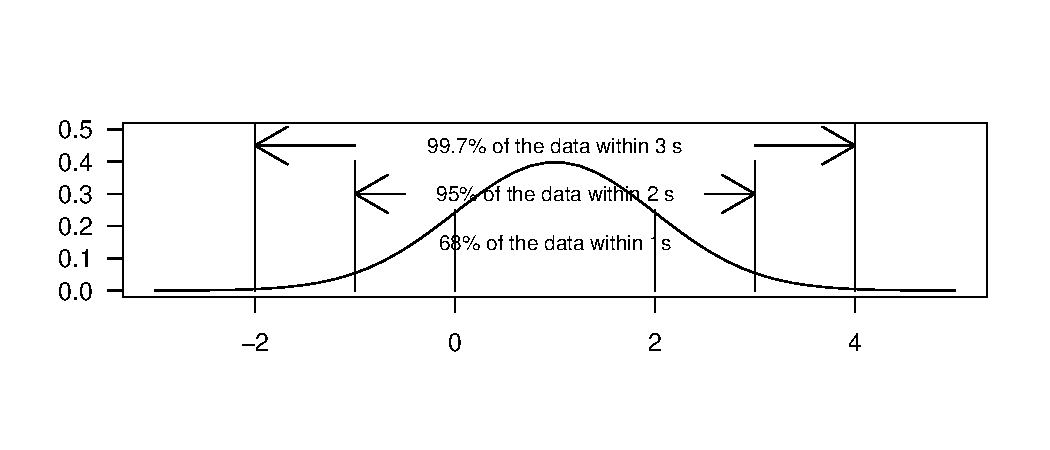
\includegraphics[width=\maxwidth]{figure/unnamed-chunk-17-1} 

\end{knitrout}
\caption{The variation of the population can be estimated with $s$, standard deviation.}
\label{fig:3rule}
\end{figure*}

When we calculate the sample mean we are usually interested not in the mean of this particular sample, but in the mean for individuals of this type---in statistical terms, of the population from which the sample comes. We usually collect data in order to generalise from them and so use the sample mean as an estimate of the mean for the whole population. Now the sample mean will vary from sample to sample; the way this variation occurs is described by the ``sampling distribution'' of the mean. We can estimate how much sample means will vary from the standard deviation of this sampling distribution, which we call the standard error (SE) of the estimate of the mean. As the standard error is a type of standard deviation, confusion is understandable. Another way of considering the \textbf{standard error is as a measure of the precision of the sample mean}.

The standard error of the sample mean depends on both the standard deviation and the sample size, by the simple relation $SE = SD/\sqrt{\textrm{sample size}}$. The standard error falls as the sample size increases, as the extent of chance variation is reduced---this idea underlies the sample size calculation for a controlled trial, for example. By contrast the standard deviation will not tend to change as we increase the size of our sample.

\section{Selecting $\alpha$: The Level of Confidence}

An important to note that the selection of the interval depends on your decision as to what level of confidence you want. Since probability ranges from 0 to 1, the confidence intervals of the parameter can also vary within this range. However, we usually are trying to constrain the confidence interval to something narrow, for example, we usually specify confidence intervals of 0.90, 0.95, and 0.99. 


In the context of a probability density function, these levels correspond to percentages of the area of the normal density curve. For example, a 95\% confidence interval includes 95\% of the normal curve's area -- the probability of observing a value outside of this area is less than 0.05. So, following standards in statistics, we use $\alpha$ to signify the as the criterion, such that

\begin{equation}
\textrm{Confidence Interval \% } = 100 * (1-\alpha)
\end{equation}

Yet, this is still ambiguous. Because the normal curve is symmetric, half of the area is in the left tail of the curve, and the other half of the area is in the right tail of the curve. Thus, if we want to generate confidence intervals that cover both tails of the curve we need to split $\alpha$ for each side of curve. Thus for a for a 95\% confidence interval, the area in each tail is equal to 0.05/2 = 0.025.\sidenote{A figure here would be helpful!} 

\section{Estimating Confidence Intervals for Waste Audit -- Preview}

\subsection{Calculating Summary Statitics}

First, we'll create summary statistics by each type of material: 

\begin{knitrout}
\definecolor{shadecolor}{rgb}{0.969, 0.969, 0.969}\color{fgcolor}\begin{kframe}
\begin{alltt}
\hlstd{Sorted.mean} \hlkwb{<-} \hlkwd{aggregate}\hlstd{(Sorted}\hlopt{$}\hlstd{Percent,}
  \hlkwc{by}\hlstd{=}\hlkwd{list}\hlstd{(}\hlkwc{Type} \hlstd{= Sorted}\hlopt{$}\hlstd{Type,}  \hlkwc{Trash_Recycle} \hlstd{= Sorted}\hlopt{$}\hlstd{Trash_Recycle),}
  \hlstd{mean)}
\hlstd{Sorted.sd} \hlkwb{<-} \hlkwd{aggregate}\hlstd{(Sorted}\hlopt{$}\hlstd{Percent,}
  \hlkwc{by}\hlstd{=}\hlkwd{list}\hlstd{(}\hlkwc{Type} \hlstd{= Sorted}\hlopt{$}\hlstd{Type,} \hlkwc{Trash_Recycle} \hlstd{= Sorted}\hlopt{$}\hlstd{Trash_Recycle),}
  \hlstd{sd)}
\hlstd{Sorted.n} \hlkwb{<-} \hlkwd{aggregate}\hlstd{(Sorted}\hlopt{$}\hlstd{Percent,}
  \hlkwc{by}\hlstd{=}\hlkwd{list}\hlstd{(}\hlkwc{Type} \hlstd{= Sorted}\hlopt{$}\hlstd{Type,} \hlkwc{Trash_Recycle} \hlstd{= Sorted}\hlopt{$}\hlstd{Trash_Recycle),}
  \hlstd{length)}
\end{alltt}
\end{kframe}
\end{knitrout}

Here's the output of one of these lines: 

\begin{knitrout}
\definecolor{shadecolor}{rgb}{0.969, 0.969, 0.969}\color{fgcolor}\begin{kframe}
\begin{alltt}
\hlstd{Sorted.mean}
\end{alltt}
\begin{verbatim}
##         Type Trash_Recycle           x
## 1  Cardboard             R 33.13571287
## 2    Compost             R  0.01949318
## 3      Glass             R 20.03979710
## 4      Metal             R  3.68737021
## 5      Paper             R  8.45764838
## 6   Plastics             R  5.39145002
## 7      Trash             R 39.45790786
## 8  Cardboard             T  8.35691793
## 9    Compost             T  4.92356044
## 10     Glass             T  3.49363016
## 11     Metal             T  0.42348864
## 12     Paper             T  0.99133653
## 13  Plastics             T  1.86514707
## 14     Trash             T 70.69710911
\end{verbatim}
\end{kframe}
\end{knitrout}

Next we'll put change the name of the variables and merge the datasets:\sidenote{Rarely do you need to do all this, but these data are a bit complicated. The example in the next section will be much eaiser to follow, so you can let your eyes glaze over the details here.}
\begin{knitrout}
\definecolor{shadecolor}{rgb}{0.969, 0.969, 0.969}\color{fgcolor}\begin{kframe}
\begin{alltt}
\hlkwd{names}\hlstd{(Sorted.sd)}\hlkwb{=} \hlkwd{c}\hlstd{(}\hlstr{"Type"}\hlstd{,} \hlstr{"Trash_Recycle"}\hlstd{,} \hlstr{"sd"}\hlstd{);} \hlkwd{head}\hlstd{(Sorted.sd)}
\end{alltt}
\begin{verbatim}
##        Type Trash_Recycle          sd
## 1 Cardboard             R 14.14448025
## 2   Compost             R  0.03898635
## 3     Glass             R 15.45730315
## 4     Metal             R  5.83196515
## 5     Paper             R  3.70017992
## 6  Plastics             R  2.02099651
\end{verbatim}
\begin{alltt}
\hlkwd{names}\hlstd{(Sorted.n)}\hlkwb{=} \hlkwd{c}\hlstd{(}\hlstr{"Type"}\hlstd{,} \hlstr{"Trash_Recycle"}\hlstd{,} \hlstr{"n"}\hlstd{);} \hlkwd{head}\hlstd{(Sorted.n)}
\end{alltt}
\begin{verbatim}
##        Type Trash_Recycle n
## 1 Cardboard             R 4
## 2   Compost             R 4
## 3     Glass             R 4
## 4     Metal             R 4
## 5     Paper             R 4
## 6  Plastics             R 4
\end{verbatim}
\begin{alltt}
\hlstd{Sorted.mean}
\end{alltt}
\begin{verbatim}
##         Type Trash_Recycle           x
## 1  Cardboard             R 33.13571287
## 2    Compost             R  0.01949318
## 3      Glass             R 20.03979710
## 4      Metal             R  3.68737021
## 5      Paper             R  8.45764838
## 6   Plastics             R  5.39145002
## 7      Trash             R 39.45790786
## 8  Cardboard             T  8.35691793
## 9    Compost             T  4.92356044
## 10     Glass             T  3.49363016
## 11     Metal             T  0.42348864
## 12     Paper             T  0.99133653
## 13  Plastics             T  1.86514707
## 14     Trash             T 70.69710911
\end{verbatim}
\begin{alltt}
\hlstd{Sorted.SEM} \hlkwb{=} \hlkwd{merge}\hlstd{(Sorted.sd, Sorted.n)}
\hlstd{Sorted.Confidence} \hlkwb{=} \hlkwd{merge}\hlstd{(Sorted.mean, Sorted.SEM)}
\hlstd{Sorted.Confidence}\hlopt{$}\hlstd{SEM} \hlkwb{=} \hlstd{Sorted.Confidence}\hlopt{$}\hlstd{sd}\hlopt{/}\hlkwd{sqrt}\hlstd{(Sorted.Confidence}\hlopt{$}\hlstd{n)}

\hlstd{Sorted.Confidence} \hlkwb{<-} \hlkwd{droplevels}\hlstd{(Sorted.Confidence)}
\end{alltt}
\end{kframe}
\end{knitrout}

In the next section, we are going to use the t-distribution to estimate our confidence intervals.

\subsection{Calculating a Parametric Confidence Interval}

To explore our waste audit data, we will determine the 95\% confidence intervals for the mean for each mean. As usual there are dozens of way to accomplish this, but for now, let's start by getting a t-statistic based on a criteria $\alpha$ value of 0.05. Since we calculate CI for the lower and upper limit, we need to split the probability in half ($\alpha/2$) and determine the intervals for 0.025 and 0.975 of the probably distribution.  

We begin by using the t-Distribution, which is a specialized case of the normal distribution (standard normal distribution that is corrected for sample size with change in the degrees of freedom).\sidenote{A figure here would be useful!}. 

\begin{equation}
\bar{x} - t_{\alpha/2, n-1}(sd/\sqrt{n}) < \mu < \bar{x} + t_{\alpha/2, n-1}(sd/\sqrt{n}) 
\end{equation}

\begin{knitrout}
\definecolor{shadecolor}{rgb}{0.969, 0.969, 0.969}\color{fgcolor}\begin{kframe}
\begin{alltt}
\hlstd{alpha} \hlkwb{=} \hlnum{0.05}
\hlstd{degfree} \hlkwb{=} \hlnum{4} \hlopt{-} \hlnum{1}
\hlkwd{qt}\hlstd{(alpha}\hlopt{/}\hlnum{2}\hlstd{, degfree)}
\end{alltt}
\begin{verbatim}
## [1] -3.182446
\end{verbatim}
\end{kframe}
\end{knitrout}



\begin{figure*}
\caption{\% material from unsorted recycling and trash mass (95\% Confidence Intevals).}
\label{fig:percent_ci}
\begin{knitrout}
\definecolor{shadecolor}{rgb}{0.969, 0.969, 0.969}\color{fgcolor}\begin{kframe}
\begin{alltt}
\hlkwd{par}\hlstd{(}\hlkwc{cex}\hlstd{=}\hlnum{1.3}\hlstd{,} \hlkwc{cex.axis}\hlstd{=}\hlnum{1}\hlstd{)}
\hlkwd{plot}\hlstd{(xvalues,} \hlkwc{ylim}\hlstd{=Ylim,} \hlkwc{xlim}\hlstd{=}\hlkwd{c}\hlstd{(}\hlnum{0.5}\hlstd{,}\hlnum{7.5}\hlstd{),}\hlkwc{ty}\hlstd{=}\hlstr{"n"}\hlstd{,} \hlkwc{xaxt}\hlstd{=}\hlstr{'none'}\hlstd{,}
    \hlkwc{xlab}\hlstd{=}\hlstr{"Type"}\hlstd{,} \hlkwc{las}\hlstd{=}\hlnum{1}\hlstd{,} \hlkwc{ylab}\hlstd{=}\hlstr{"% of Unsorted Mass"}\hlstd{)}
\hlkwd{axis}\hlstd{(}\hlkwc{side}\hlstd{=}\hlnum{1}\hlstd{,} \hlkwc{at}\hlstd{=}\hlnum{1}\hlopt{:}\hlnum{7}\hlstd{,} \hlkwc{label}\hlstd{=}\hlkwd{levels}\hlstd{(Sorted.Confidence}\hlopt{$}\hlstd{Type),}
    \hlkwc{cex.axis}\hlstd{=}\hlnum{.5}\hlstd{)}
\hlkwd{points}\hlstd{(xvalues,}
    \hlstd{Sorted.Confidence}\hlopt{$}\hlstd{x[Sorted.Confidence}\hlopt{$}\hlstd{Trash_Recycle}\hlopt{==}\hlstr{"R"}\hlstd{],}
    \hlkwc{col}\hlstd{=}\hlstr{"darkgreen"}\hlstd{,} \hlkwc{pch}\hlstd{=}\hlnum{19}\hlstd{)}
\hlkwd{points}\hlstd{(x1, Sorted.Confidence}\hlopt{$}\hlstd{x[Sorted.Confidence}\hlopt{$}\hlstd{Trash_Recycle}\hlopt{==}\hlstr{"T"}\hlstd{],}
    \hlkwc{col}\hlstd{=}\hlstr{"Red"}\hlstd{,} \hlkwc{pch}\hlstd{=}\hlnum{2}\hlstd{)}
\hlkwd{with}\hlstd{(Sorted.Confidence[Sorted.Confidence}\hlopt{$}\hlstd{Trash_Recycle}\hlopt{==}\hlstr{"R"}\hlstd{,],}
     \hlkwd{arrows}\hlstd{(xvalues, CI.low, xvalues, CI.high,} \hlkwc{length}\hlstd{=}\hlnum{0.05}\hlstd{,}
            \hlkwc{angle}\hlstd{=}\hlnum{90}\hlstd{,} \hlkwc{code}\hlstd{=}\hlnum{3}\hlstd{,} \hlkwc{lwd}\hlstd{=}\hlnum{2}\hlstd{,} \hlkwc{col}\hlstd{=}\hlstr{"darkgreen"}\hlstd{))}
\hlkwd{with}\hlstd{(Sorted.Confidence[Sorted.Confidence}\hlopt{$}\hlstd{Trash_Recycle}\hlopt{==}\hlstr{"T"}\hlstd{,],}
     \hlkwd{arrows}\hlstd{(x1, CI.low, x1, CI.high,} \hlkwc{length}\hlstd{=}\hlnum{0.05}\hlstd{,}
            \hlkwc{angle}\hlstd{=}\hlnum{90}\hlstd{,} \hlkwc{code}\hlstd{=}\hlnum{3}\hlstd{,} \hlkwc{lwd}\hlstd{=}\hlnum{2}\hlstd{,} \hlkwc{col}\hlstd{=}\hlstr{"red"}\hlstd{))}
\hlcom{# Add a legend}
\hlkwd{legend}\hlstd{(}\hlnum{2}\hlstd{,} \hlnum{95}\hlstd{,} \hlkwc{legend}\hlstd{=}\hlkwd{c}\hlstd{(}\hlstr{"Recycling"}\hlstd{,} \hlstr{"Trash"}\hlstd{),}
       \hlkwc{col}\hlstd{=}\hlkwd{c}\hlstd{(}\hlstr{"darkgreen"}\hlstd{,} \hlstr{"red"}\hlstd{),} \hlkwc{pch}\hlstd{=}\hlkwd{c}\hlstd{(}\hlnum{19}\hlstd{,} \hlnum{2}\hlstd{),} \hlkwc{cex}\hlstd{=}\hlnum{.8}\hlstd{,} \hlkwc{bty}\hlstd{=}\hlstr{'n'}\hlstd{)}
\end{alltt}
\end{kframe}
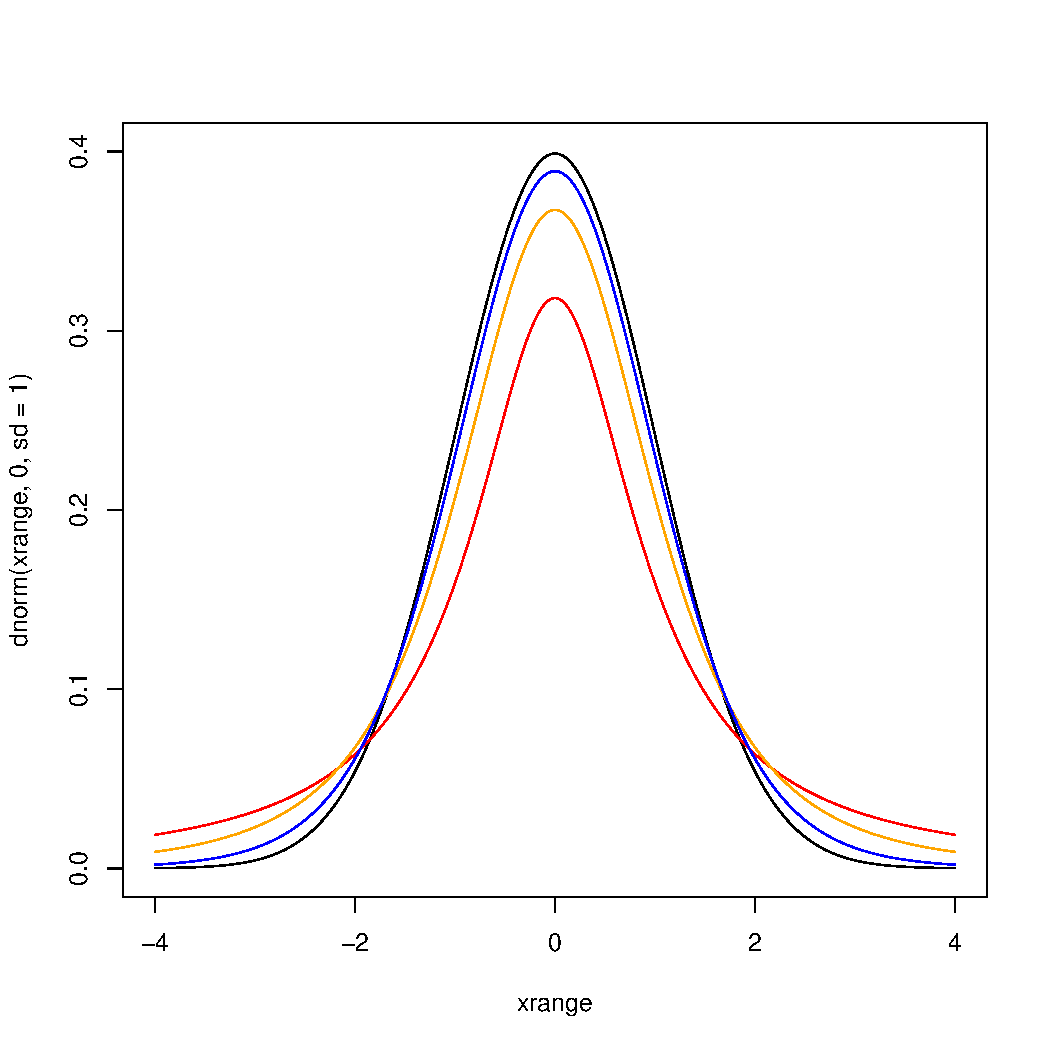
\includegraphics[width=\maxwidth]{figure/unnamed-chunk-22-1} 

\end{knitrout}
\end{figure*}


\section{Implementing Code to Create Confidence Intervals}

\subsection{Steps to Create Confidence Intervals}

This example assumes that the samples are drawn from a Normal distribution. The basic procedure for calculating a confidence interval for a population mean is as follows:
\begin{enumerate}
  \item Identify the sample mean, $\bar{x}$.
  
  \item Identify whether the population standard deviation is known, $\sigma$, or is unknown and is estimated by the sample standard deviation $s$.
  
  \begin{itemize}
    \item If the population standard deviation is known then $z^{*}=\Phi ^{-1}\left(1-{\frac {\alpha }{2}}\right)=-\Phi ^{-1}\left({\frac {\alpha }{2}}\right)$, where $C=100(1-\alpha)$ is the confidence level and $\Phi$  is the CDF of the standard normal distribution, used as the critical value. This value is only dependent on the confidence level for the test. Typical two sided confidence levels are:
    
\begin{table}
\begin{tabular}{ll}
C	    & z* \\ \hline
99\%	  & 2.576 \\
98\%	  & 2.326 \\
95\%	  & 1.96 \\
90\%	  & 1.645 \\
\end{tabular}
\end{table}

\item If the population standard deviation is unknown then the Student's t distribution is used as the critical value. This value is dependent on the confidence level ($C$) for the test and degrees of freedom. The degrees of freedom are found by subtracting one from the number of observations, $n − 1$. The critical value is found from the t-distribution table. In this table the critical value is written as $t^{*}=t_{\alpha }(r)$, where $r$ is the degrees of freedom and $\alpha ={1-C \over 2}$.

  \end{itemize}

\item Plug the found values into the appropriate equations:

\begin{itemize}
  \item For a known standard deviation: $\left({\bar {x}}-z^{*}{\sigma \over {\sqrt {n}}},{\bar {x}}+z^{*}{\sigma \over {\sqrt {n}}}\right)$

  \item For an unknown standard deviation: $\displaystyle \left({\bar {x}}-t^{*}{s \over {\sqrt {n}}},{\bar {x}}+t^{*}{s \over {\sqrt {n}}}\right)$
\end{itemize}

\end{enumerate}


\subsection{Normal versus the t-Distribution}

For demonstration purposes, we should compare the standard normal distribution to the t-distribuition so we understand what the implications of distribution might mean in hypothesis testing!

\begin{figure}
\begin{knitrout}
\definecolor{shadecolor}{rgb}{0.969, 0.969, 0.969}\color{fgcolor}\begin{kframe}
\begin{alltt}
\hlstd{xrange} \hlkwb{=} \hlkwd{seq}\hlstd{(}\hlopt{-}\hlnum{4}\hlstd{,} \hlnum{4}\hlstd{,} \hlkwc{by}\hlstd{=}\hlnum{.02}\hlstd{)}
\hlkwd{plot}\hlstd{(xrange,} \hlkwd{dnorm}\hlstd{(xrange,} \hlnum{0}\hlstd{,} \hlkwc{sd}\hlstd{=}\hlnum{1}\hlstd{),} \hlkwc{ty}\hlstd{=}\hlstr{'l'}\hlstd{,} \hlkwc{ylim}\hlstd{=}\hlkwd{c}\hlstd{(}\hlnum{0}\hlstd{,}\hlnum{.4}\hlstd{),} \hlkwc{xlim}\hlstd{=}\hlkwd{c}\hlstd{(}\hlopt{-}\hlnum{4}\hlstd{,}\hlnum{4}\hlstd{))}

\hlkwd{lines}\hlstd{(xrange,} \hlkwd{dt}\hlstd{(xrange,} \hlkwc{df}\hlstd{=}\hlnum{1}\hlstd{),} \hlkwc{ty}\hlstd{=}\hlstr{'l'}\hlstd{,} \hlkwc{col}\hlstd{=}\hlstr{'red'}\hlstd{)}
\hlkwd{lines}\hlstd{(xrange,} \hlkwd{dt}\hlstd{(xrange,} \hlkwc{df}\hlstd{=}\hlnum{3}\hlstd{),} \hlkwc{ty}\hlstd{=}\hlstr{'l'}\hlstd{,} \hlkwc{col}\hlstd{=}\hlstr{'orange'}\hlstd{)}
\hlkwd{lines}\hlstd{(xrange,} \hlkwd{dt}\hlstd{(xrange,} \hlkwc{df}\hlstd{=}\hlnum{10}\hlstd{),} \hlkwc{ty}\hlstd{=}\hlstr{'l'}\hlstd{,} \hlkwc{col}\hlstd{=}\hlstr{'blue'}\hlstd{)}
\end{alltt}
\end{kframe}
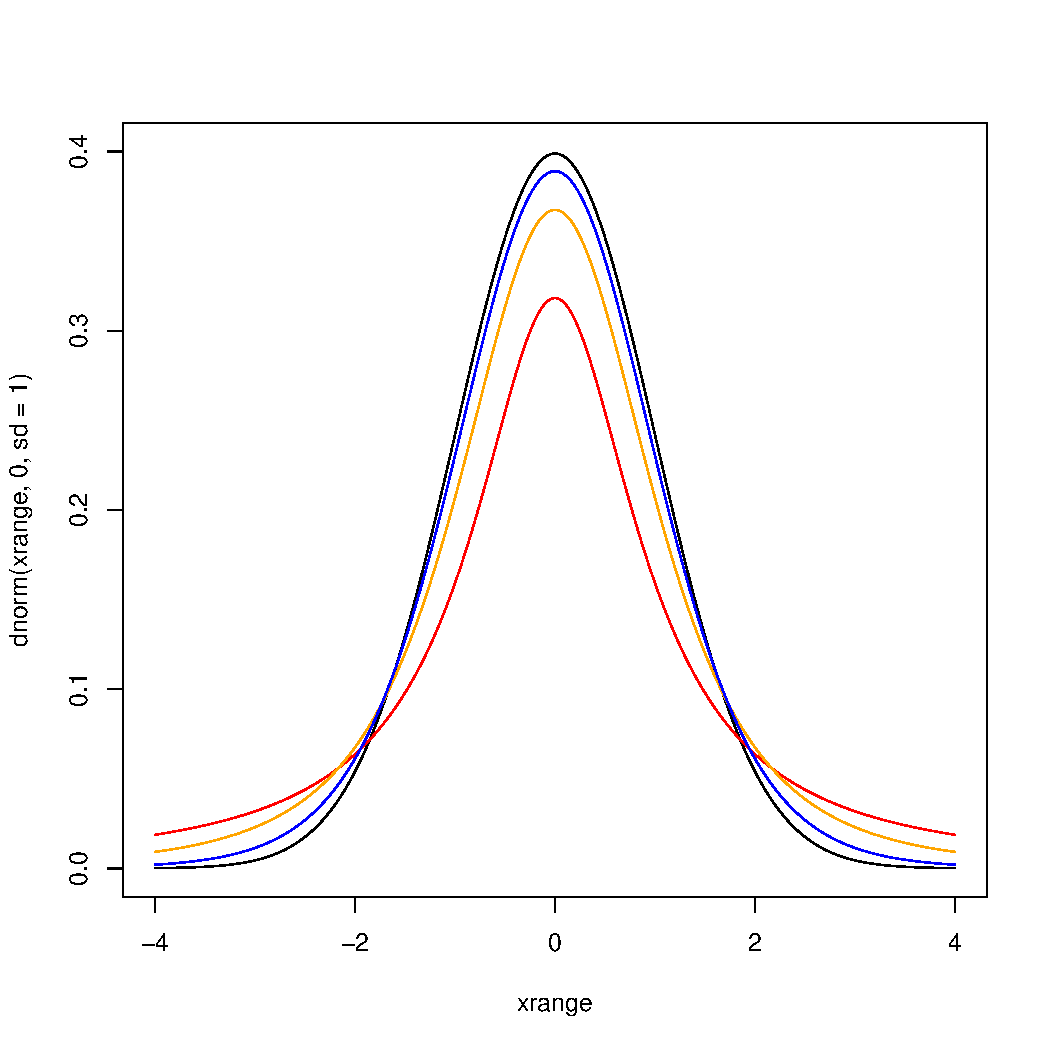
\includegraphics[width=\maxwidth]{figure/unnamed-chunk-23-1} 

\end{knitrout}
\end{figure}

Notice that the t-distribution is squatter in the middle and fatter at the edges. This means there is more probability ``area'' at the ends. But as you approach the n=20, the curves are increasingly overlapping.

\subsection{How to make these plots}

Notice that I used \texttt{dnorm()} and \texttt{dt()} functions to create the figures. What are these? These functions create probability density curves. It's cool to see that that there are several variants of these functions that are related. 

\begin{description}
  \item[\texttt{rnorm()}] generates n random numbers from a normal distribution with a defined mean and sd (standard deviation).
  \item[\texttt{dnorm()}] generates probability densities based on the quantile, mean, and sd. This can be based on an upper or lower side of the distribution. More on this below.
  \item[\texttt{qnorm()}] generates quantiles based on the probabilities, mean and sd. This can also be based on the upper or lower side of the distribution. 
  \item[\texttt{pnorm()}] generates probabilities based on the quantiles, mean and sd.
\end{description}

\noindent To test demonstrate these functions, let's try each out. First, I'll create a set of five random numbers (let's use the standard normal, which as a mean of zero and a sd of one) and round them to the nearest 10th. 

\begin{knitrout}
\definecolor{shadecolor}{rgb}{0.969, 0.969, 0.969}\color{fgcolor}\begin{kframe}
\begin{alltt}
(randomnumbers = \hlkwd{round}(\hlkwd{rnorm}(5, mean=0, sd=1), 0.1)
\hlcom{#hist(randomnumbers)}
\end{alltt}


{\ttfamily\noindent\bfseries\color{errorcolor}{\#\# Error: <text>:3:0: unexpected end of input\\\#\# 1: (randomnumbers = round(rnorm(5, mean=0, sd=1), 0.1)\\\#\# 2: \#hist(randomnumbers)\\\#\#\ \  \textasciicircum{}}}\end{kframe}
\end{knitrout}

Now, let's uses these figure out what the probabilies, using the default for lower tail, i.e. \texttt{lower.tail=T}. In other words, what is the probability that the number will be higher than the lower side of the tail. 

\begin{knitrout}
\definecolor{shadecolor}{rgb}{0.969, 0.969, 0.969}\color{fgcolor}\begin{kframe}
\begin{alltt}
\hlkwd{round}\hlstd{(}\hlkwd{pnorm}\hlstd{(randomnumbers,} \hlkwc{mean}\hlstd{=}\hlnum{0}\hlstd{,} \hlkwc{sd}\hlstd{=}\hlnum{1}\hlstd{,} \hlkwc{lower.tail}\hlstd{=T),} \hlnum{2}\hlstd{)}
\end{alltt}


{\ttfamily\noindent\bfseries\color{errorcolor}{\#\# Error in pnorm(randomnumbers, mean = 0, sd = 1, lower.tail = T): object 'randomnumbers' not found}}\end{kframe}
\end{knitrout}

finally, let's see what the qauntiles look like based on various probabilities

\begin{knitrout}
\definecolor{shadecolor}{rgb}{0.969, 0.969, 0.969}\color{fgcolor}\begin{kframe}
\begin{alltt}
\hlkwd{round}\hlstd{(}\hlkwd{qnorm}\hlstd{(}\hlkwd{c}\hlstd{(}\hlnum{0.01}\hlstd{,} \hlnum{0.025}\hlstd{,} \hlnum{.05}\hlstd{,} \hlnum{.1}\hlstd{,} \hlnum{.5}\hlstd{,} \hlnum{.9}\hlstd{,} \hlnum{.95}\hlstd{,} \hlnum{.975}\hlstd{,} \hlnum{0.99}\hlstd{),}
            \hlkwc{mean}\hlstd{=}\hlnum{0}\hlstd{,} \hlkwc{sd}\hlstd{=}\hlnum{1}\hlstd{,} \hlkwc{lower.tail}\hlstd{=T),} \hlnum{2}\hlstd{)}
\end{alltt}
\begin{verbatim}
## [1] -2.33 -1.96 -1.64 -1.28  0.00  1.28  1.64  1.96  2.33
\end{verbatim}
\end{kframe}
\end{knitrout}

If we switch these numbers to the 68-95-99.7 rule probabilies. First, we need to divide the tails in 1/2 and then we can put them in the \texttt{qnorm()} function. We can see where the the 1, 2 and 3 standard deviations came from (rounded right?). Pretty Neat!

\begin{knitrout}
\definecolor{shadecolor}{rgb}{0.969, 0.969, 0.969}\color{fgcolor}\begin{kframe}
\begin{alltt}
\hlstd{percent.68} \hlkwb{=} \hlstd{(}\hlnum{1} \hlopt{-} \hlnum{0.68}\hlstd{)}\hlopt{/}\hlnum{2}
\hlstd{percent.95} \hlkwb{<-} \hlstd{(}\hlnum{1} \hlopt{-} \hlnum{0.95}\hlstd{)}\hlopt{/}\hlnum{2}
\hlstd{percent.99} \hlkwb{<-} \hlstd{(}\hlnum{1} \hlopt{-} \hlnum{0.997}\hlstd{)}\hlopt{/}\hlnum{2}
\hlkwd{round}\hlstd{(}\hlopt{-}\hlkwd{qnorm}\hlstd{(}\hlkwd{c}\hlstd{(percent.68, percent.95, percent.99),} \hlkwc{mean}\hlstd{=}\hlnum{0}\hlstd{,} \hlkwc{sd}\hlstd{=}\hlnum{1}\hlstd{),} \hlnum{2}\hlstd{)}
\end{alltt}
\begin{verbatim}
## [1] 0.99 1.96 2.97
\end{verbatim}
\end{kframe}
\end{knitrout}


\subsection{Calculating Confidence Intervals with known $\sigma^2$.}

Because we have the values for the entire population, we can estimate confidence intervals using the normal distribution (z* scores) using the formula above. 

We'll create confidence intervals using our $n$=100 sample. 

The $\bar{x}$ = 10.11 and $\sigma$ = 0.993148. First, we'll create a function to calculate our confidence intervals that has the following inputs: sample vector, level of confidence ($\alpha$), and $\mu$.

\begin{knitrout}
\definecolor{shadecolor}{rgb}{0.969, 0.969, 0.969}\color{fgcolor}\begin{kframe}
\begin{alltt}
\hlstd{cl}\hlkwb{<-} \hlkwa{function}\hlstd{(}\hlkwc{sample}\hlstd{,} \hlkwc{alpha}\hlstd{,} \hlkwc{sigma}\hlstd{)\{}
  \hlstd{sem} \hlkwb{<-} \hlstd{sigma}\hlopt{/}\hlkwd{sqrt}\hlstd{(}\hlkwd{length}\hlstd{(sample))}
  \hlstd{ucl} \hlkwb{<-} \hlkwd{mean}\hlstd{(sample)} \hlopt{+} \hlkwd{qnorm}\hlstd{(}\hlnum{1}\hlopt{-}\hlstd{alpha}\hlopt{/}\hlnum{2}\hlstd{)}\hlopt{*}\hlstd{sem}
  \hlstd{lcl} \hlkwb{<-} \hlkwd{mean}\hlstd{(sample)} \hlopt{-} \hlkwd{qnorm}\hlstd{(}\hlnum{1}\hlopt{-}\hlstd{alpha}\hlopt{/}\hlnum{2}\hlstd{)}\hlopt{*}\hlstd{sem}
  \hlstd{ci} \hlkwb{<-} \hlkwd{c}\hlstd{(lcl, ucl)}
  \hlkwd{return}\hlstd{(ci)}
\hlstd{\}}

\hlstd{(cl95.n100} \hlkwb{<-} \hlkwd{cl}\hlstd{(n100,} \hlnum{0.05}\hlstd{,} \hlkwd{sd}\hlstd{(N1000)))}
\end{alltt}
\begin{verbatim}
## [1]  9.911347 10.300653
\end{verbatim}
\begin{alltt}
\hlstd{xvalues} \hlkwb{=} \hlkwd{seq}\hlstd{(}\hlnum{6}\hlstd{,}\hlnum{14}\hlstd{,}\hlnum{.1}\hlstd{)}
\hlkwd{plot}\hlstd{(xvalues,} \hlkwd{dnorm}\hlstd{(xvalues,} \hlkwd{mean}\hlstd{(n100),} \hlkwd{sd}\hlstd{(n100)),} \hlkwc{ty}\hlstd{=}\hlstr{'l'}\hlstd{)}
\hlkwd{abline}\hlstd{(}\hlkwc{v}\hlstd{=}\hlkwd{mean}\hlstd{(n100))}
\hlkwd{abline}\hlstd{(}\hlkwc{v}\hlstd{=cl95.n100[}\hlnum{1}\hlstd{],} \hlkwc{col}\hlstd{=}\hlstr{'grey'}\hlstd{)}
\hlkwd{abline}\hlstd{(}\hlkwc{v}\hlstd{=cl95.n100[}\hlnum{2}\hlstd{],} \hlkwc{col}\hlstd{=}\hlstr{'grey'}\hlstd{)}
\end{alltt}
\end{kframe}
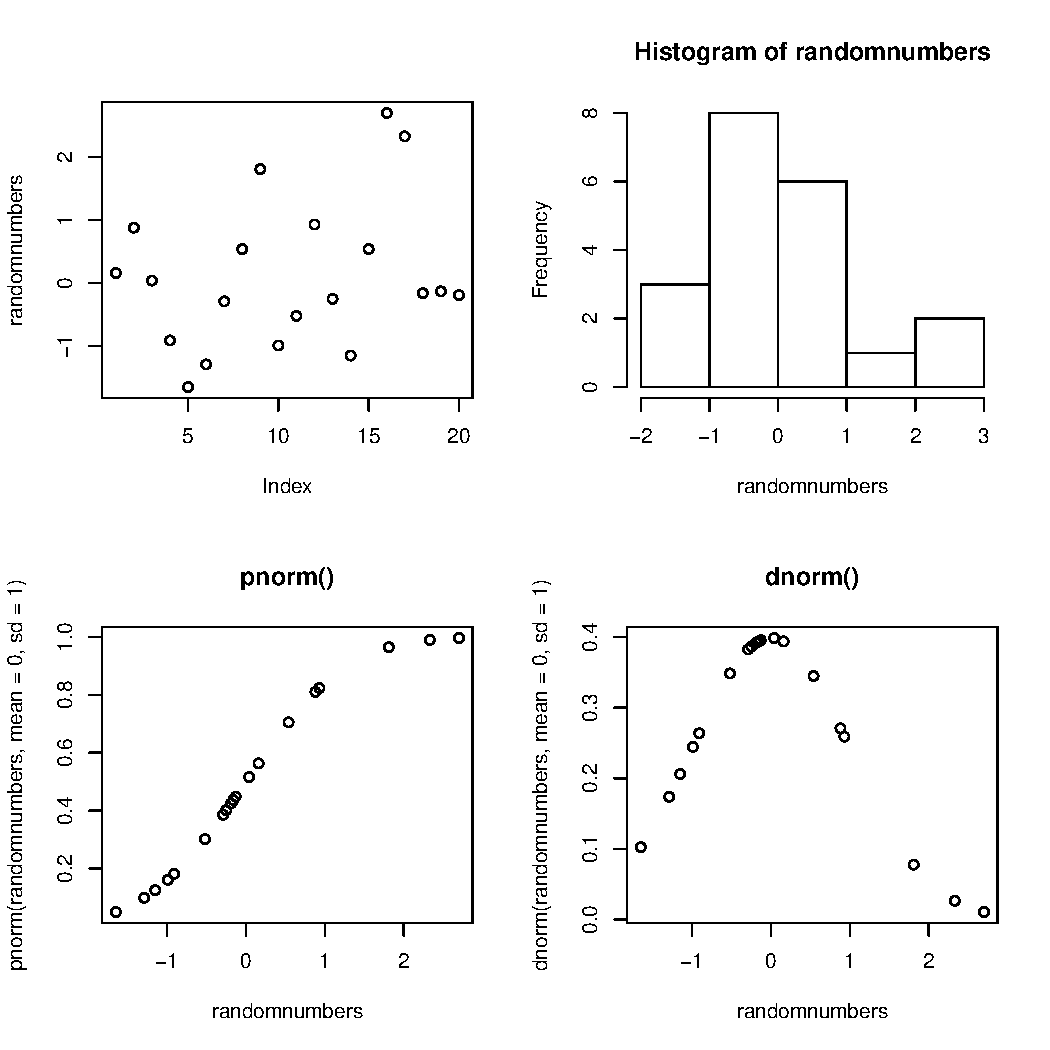
\includegraphics[width=\maxwidth]{figure/unnamed-chunk-27-1} 

\end{knitrout}

\section{How does n influence confidence intervals?}

\begin{knitrout}
\definecolor{shadecolor}{rgb}{0.969, 0.969, 0.969}\color{fgcolor}\begin{kframe}
\begin{alltt}
\hlstd{(cl95.n20} \hlkwb{<-} \hlkwd{cl}\hlstd{(n20,} \hlnum{0.05}\hlstd{,} \hlkwd{sd}\hlstd{(N1000)))}
\end{alltt}
\begin{verbatim}
## [1]  9.764742 10.635258
\end{verbatim}
\begin{alltt}
\hlstd{(cl95.n20} \hlkwb{<-} \hlkwd{cl}\hlstd{(n20,} \hlnum{0.05}\hlstd{,} \hlkwd{sd}\hlstd{(N1000)))}
\end{alltt}
\begin{verbatim}
## [1]  9.764742 10.635258
\end{verbatim}
\begin{alltt}
\hlstd{(cl95.n5} \hlkwb{<-} \hlkwd{cl}\hlstd{(n5,} \hlnum{0.05}\hlstd{,} \hlkwd{sd}\hlstd{(N1000)))}
\end{alltt}
\begin{verbatim}
## [1]  8.809483 10.550517
\end{verbatim}
\begin{alltt}
\hlstd{xvalues} \hlkwb{=} \hlkwd{seq}\hlstd{(}\hlnum{6}\hlstd{,}\hlnum{14}\hlstd{,}\hlnum{.1}\hlstd{)}
\hlkwd{plot}\hlstd{(xvalues,} \hlkwd{dnorm}\hlstd{(xvalues,} \hlkwd{mean}\hlstd{(n100),} \hlkwd{sd}\hlstd{(n100)),} \hlkwc{ty}\hlstd{=}\hlstr{'l'}\hlstd{,} \hlkwc{col}\hlstd{=}\hlstr{'green'}\hlstd{,} \hlkwc{ylim}\hlstd{=}\hlkwd{c}\hlstd{(}\hlnum{0}\hlstd{,} \hlnum{0.6}\hlstd{))}
\hlkwd{abline}\hlstd{(}\hlkwc{v}\hlstd{=}\hlkwd{mean}\hlstd{(n100),} \hlkwc{col}\hlstd{=}\hlstr{'green'}\hlstd{)}
\hlkwd{abline}\hlstd{(}\hlkwc{v}\hlstd{=cl95.n100[}\hlnum{1}\hlstd{],} \hlkwc{col}\hlstd{=}\hlstr{'green'}\hlstd{)}
\hlkwd{abline}\hlstd{(}\hlkwc{v}\hlstd{=cl95.n100[}\hlnum{2}\hlstd{],} \hlkwc{col}\hlstd{=}\hlstr{'green'}\hlstd{)}

\hlkwd{lines}\hlstd{(xvalues,} \hlkwd{dnorm}\hlstd{(xvalues,} \hlkwd{mean}\hlstd{(n20),} \hlkwd{sd}\hlstd{(n20)),} \hlkwc{ty}\hlstd{=}\hlstr{'l'}\hlstd{,} \hlkwc{col}\hlstd{=}\hlstr{'blue'}\hlstd{)}
\hlkwd{abline}\hlstd{(}\hlkwc{v}\hlstd{=cl95.n20[}\hlnum{1}\hlstd{],} \hlkwc{col}\hlstd{=}\hlstr{'blue'}\hlstd{)}
\hlkwd{abline}\hlstd{(}\hlkwc{v}\hlstd{=cl95.n20[}\hlnum{2}\hlstd{],} \hlkwc{col}\hlstd{=}\hlstr{'blue'}\hlstd{)}

\hlkwd{lines}\hlstd{(xvalues,} \hlkwd{dnorm}\hlstd{(xvalues,} \hlkwd{mean}\hlstd{(n5),} \hlkwd{sd}\hlstd{(n5)),} \hlkwc{ty}\hlstd{=}\hlstr{'l'}\hlstd{,} \hlkwc{col}\hlstd{=}\hlstr{'red'}\hlstd{)}
\hlkwd{abline}\hlstd{(}\hlkwc{v}\hlstd{=cl95.n5[}\hlnum{1}\hlstd{],} \hlkwc{col}\hlstd{=}\hlstr{'red'}\hlstd{)}
\hlkwd{abline}\hlstd{(}\hlkwc{v}\hlstd{=cl95.n5[}\hlnum{2}\hlstd{],} \hlkwc{col}\hlstd{=}\hlstr{'red'}\hlstd{)}
\end{alltt}
\end{kframe}
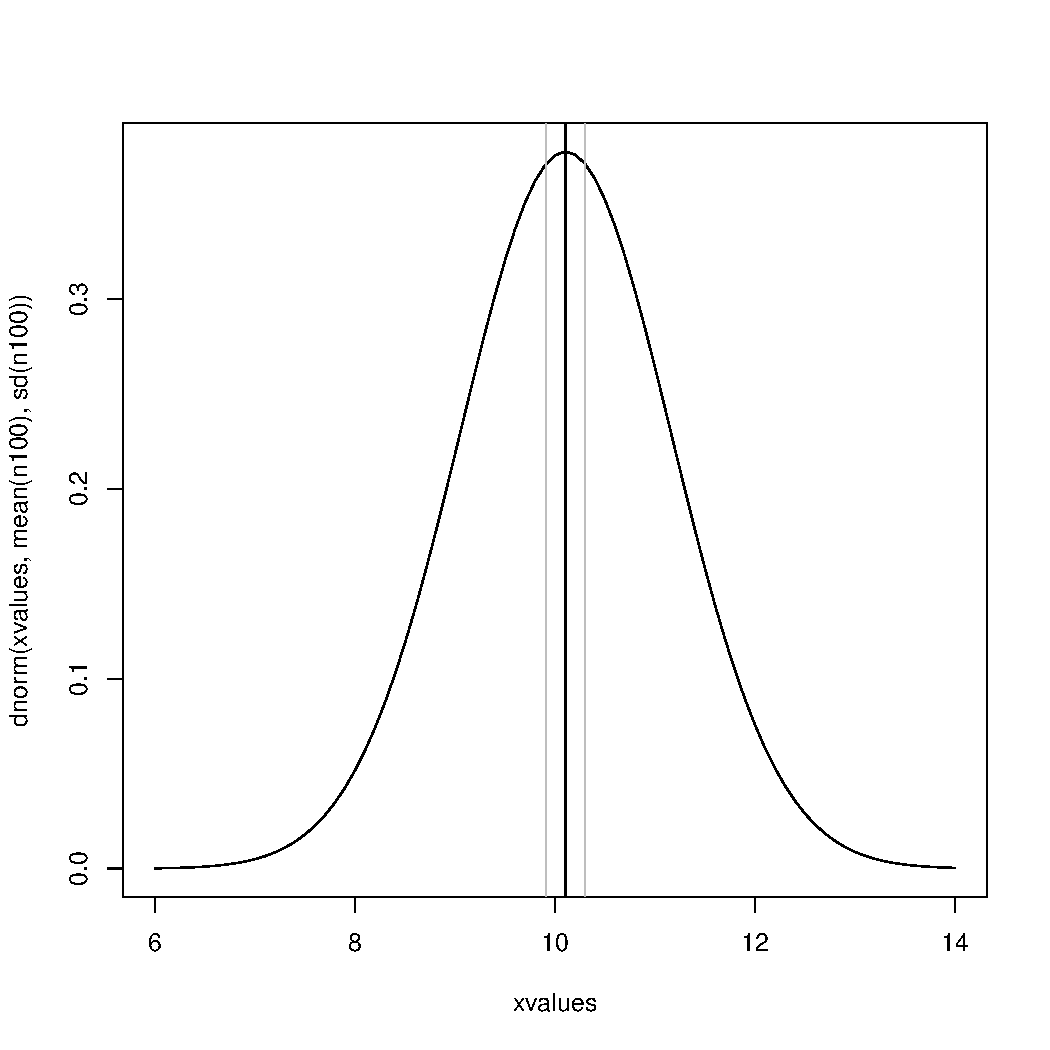
\includegraphics[width=\maxwidth]{figure/unnamed-chunk-28-1} 

\end{knitrout}

\subsection{Confidence Intervals with an unknown $\sigma$}

\begin{knitrout}
\definecolor{shadecolor}{rgb}{0.969, 0.969, 0.969}\color{fgcolor}\begin{kframe}
\begin{alltt}
\hlkwd{qt}\hlstd{((}\hlnum{1}\hlopt{-}\hlnum{.95}\hlstd{)}\hlopt{/}\hlnum{2}\hlstd{,} \hlnum{4}\hlstd{)}\hlopt{*}\hlkwd{sd}\hlstd{(n5)}\hlopt{/}\hlkwd{sqrt}\hlstd{(}\hlnum{5}\hlstd{)}\hlopt{+}\hlkwd{mean}\hlstd{(n5)}
\end{alltt}
\begin{verbatim}
## [1] 8.761672
\end{verbatim}
\end{kframe}
\end{knitrout}
@

\subsection{Misunderstandings about Confidence Intervals}

Confidence intervals and levels are frequently misunderstood, and published studies have shown that even professional scientists often misinterpret them. I find myself tripped up the the vocabularly regularly. 

A 95\% confidence level does not mean that for a given realized interval there is a 95\% probability that the population parameter lies within the interval (i.e., a 95\% probability that the interval covers the population parameter). According to the strict frequentist interpretation, once an interval is calculated, this interval either covers the parameter value or it does not; it is no longer a matter of probability. 

The 95\% probability relates to \textbf{the reliability of the estimation procedure}, not to a specific calculated interval.

Neyman himself (the original proponent of confidence intervals) made this point in his original paper:

\begin{quote}
It will be noticed that in the above description, the probability statements refer to the problems of estimation with which the statistician will be concerned in the future. In fact, I have repeatedly stated that the frequency of correct results will tend to $\alpha$. Consider now the case when a sample is already drawn, and the calculations have given [particular limits]. Can we say that in this particular case the probability of the true value [falling between these limits] is equal to $\alpha$? The answer is obviously in the negative. The parameter is an unknown constant, and no probability statement concerning its value may be made \ldots
\end{quote}

\noindent Deborah Mayo expands on this further as follows:

\begin{quote}
It must be stressed, however, that having seen the value [of the data], Neyman-Pearson theory never permits one to conclude that the specific confidence interval formed covers the true value of 0 with either $(1 - \alpha)100\%$ probability or $(1 - \alpha)100\%$ degree of confidence. Seidenfeld's remark seems rooted in a (not uncommon) desire for Neyman-Pearson confidence intervals to provide something which they cannot legitimately provide; namely, a measure of the degree of probability, belief, or support that an unknown parameter value lies in a specific interval. Following Savage (1962), the probability that a parameter lies in a specific interval may be referred to as a measure of final precision. While a measure of final precision may seem desirable, and while confidence levels are often (wrongly) interpreted as providing such a measure, no such interpretation is warranted. Admittedly, such a misinterpretation is encouraged by the word 'confidence.'
\end{quote}

\begin{itemize}
  \item A 95\% confidence level does not mean that 95\% of the sample data lie within the confidence interval.
  \item A confidence interval is not a definitive range of plausible values for the sample parameter, though it may be understood as an estimate of plausible values for the population parameter.
  \item A particular confidence level of 95\% calculated from an experiment does not mean that there is a 95\% probability of a sample parameter from a repeat of the experiment falling within this interval.
\end{itemize}

\subsection{What what the heck is a confidence interval?}

Various interpretations of a confidence interval can be given (taking the 90\% confidence interval as an example in the following).

\begin{itemize}
  \item The confidence interval can be expressed in terms of samples (or repeated samples): ``Were this procedure to be repeated on numerous samples, the fraction of calculated confidence intervals (which would differ for each sample) that encompass the true population parameter would tend toward 90\%.''

  \item The confidence interval can be expressed in terms of a single sample: ``There is a 90\% probability that the calculated confidence interval from some future experiment encompasses the true value of the population parameter.'' Note this is a probability statement about the confidence interval, not the population parameter. This considers the probability associated with a confidence interval from a pre-experiment point of view, in the same context in which arguments for the random allocation of treatments to study items are made. Here the experimenter sets out the way in which they intend to calculate a confidence interval and to know, before they do the actual experiment, that the interval they will end up calculating has a particular chance of covering the true but unknown value. This is very similar to the ``repeated sample'' interpretation above, except that it avoids relying on considering hypothetical repeats of a sampling procedure that may not be repeatable in any meaningful sense.

  \item The explanation of a confidence interval can amount to something like: ``The confidence interval represents values for the population parameter for which the difference between the parameter and the observed estimate is not statistically significant at the 10\% level.'' In fact, this relates to one particular way in which a confidence interval may be constructed.

\end{itemize}

In each of the above, the following applies: If the true value of the parameter lies outside the 90\% confidence interval, then a sampling event has occurred which had a probability of 10\% (or less) of happening by chance.



\clearpage
\section{t-test}

\subsection{What is a (statisical) hypothesis?}

A hypothesis is a prediction --- and using the frequentists approach, we make a negative prediction, i.e. that there is no pattern, to test. In our example with the waste, we can test was the the amount recycling stastically significant compared to the total waste. In other words, were students diverting waste. We can test if the confidence intervals include 100\%. 

First, we'll subset the data!
\begin{knitrout}
\definecolor{shadecolor}{rgb}{0.969, 0.969, 0.969}\color{fgcolor}\begin{kframe}
\begin{alltt}
\hlstd{trash} \hlkwb{=} \hlkwd{subset}\hlstd{(Sorted, Type} \hlopt{==} \hlstr{"Trash"}\hlstd{,}
        \hlkwc{select} \hlstd{=} \hlkwd{c}\hlstd{(Trash_Recycle, Type, Percent)); trash}
\end{alltt}
\begin{verbatim}
##    Trash_Recycle  Type  Percent
## 8              R Trash 24.95127
## 16             R Trash 33.24468
## 24             R Trash 31.60622
## 32             R Trash 68.02947
## 40             T Trash 48.70641
## 48             T Trash 73.69888
## 56             T Trash 78.74251
## 64             T Trash 81.64062
\end{verbatim}
\end{kframe}
\end{knitrout}

\begin{knitrout}
\definecolor{shadecolor}{rgb}{0.969, 0.969, 0.969}\color{fgcolor}\begin{kframe}
\begin{alltt}
\hlkwd{t.test}\hlstd{(trash[}\hlnum{1}\hlopt{:}\hlnum{4}\hlstd{,}\hlnum{3}\hlstd{],} \hlkwc{mu}\hlstd{=}\hlnum{100}\hlstd{)}
\end{alltt}
\begin{verbatim}
## 
## 	One Sample t-test
## 
## data:  trash[1:4, 3]
## t = -6.2471, df = 3, p-value = 0.008275
## alternative hypothesis: true mean is not equal to 100
## 95 percent confidence interval:
##   8.616218 70.299597
## sample estimates:
## mean of x 
##  39.45791
\end{verbatim}
\end{kframe}
\end{knitrout}

The t.test output is a bit confusioning. But let's start with the null hypothesis, which is the mean is equal to 100. The alternative is ``true mean is not equal to 100.'' Next, let's check out the p-value: 0.0083.\sidenote{What should you report?  We don't need all these decimals!  Thus, we usually report p values as < 0.05, <0.01, and <0.001. It's a good practices and sufficiently informative for most purposes.}

Thus, we can reject the null hypothesis, the mean is equal to 100\%. Thus, we are testing if there is a difference between the total unsorted weight of the recyling and the weight of the trash in the recycling bins. We hope there is a difference! And there is because we can reject the null hypothesis. 

Thus, evidence students are diverting not just dumping stuff randomly in the recycling bins. I guess that is good news!

A second question is what there a signficant amount of recyclable material that should have been recycled?  What the amount of potentially diverted material statistically significant?

\begin{knitrout}
\definecolor{shadecolor}{rgb}{0.969, 0.969, 0.969}\color{fgcolor}\begin{kframe}
\begin{alltt}
\hlkwd{t.test}\hlstd{(trash[}\hlnum{5}\hlopt{:}\hlnum{8}\hlstd{,}\hlnum{3}\hlstd{],} \hlkwc{mu}\hlstd{=}\hlnum{100}\hlstd{)}
\end{alltt}
\begin{verbatim}
## 
## 	One Sample t-test
## 
## data:  trash[5:8, 3]
## t = -3.901, df = 3, p-value = 0.0299
## alternative hypothesis: true mean is not equal to 100
## 95 percent confidence interval:
##  46.79183 94.60239
## sample estimates:
## mean of x 
##  70.69711
\end{verbatim}
\end{kframe}
\end{knitrout}

This is not surprising, but disappointing. The amount of recycling in the trash is significantly below 100\%, that suggests recyclelable materials are being put into the trash in a signficant fashion. We might notice that one observation \# is a big problem. What is \#40?

\begin{knitrout}
\definecolor{shadecolor}{rgb}{0.969, 0.969, 0.969}\color{fgcolor}\begin{kframe}
\begin{alltt}
\hlstd{Sorted[}\hlnum{35}\hlstd{,]} \hlcom{# Not sure why this isn't #40, still sorting that out... !!!}
\end{alltt}
\begin{verbatim}
##    Sample.Date Trash_Recycle Location  Type Mass_Container
## 40   9/23/2019             T Dialynas Trash           43.3
##    Container NetMass Total  Percent
## 40         0    43.3  88.9 48.70641
\end{verbatim}
\end{kframe}
\end{knitrout}

No surprise -- the parties is Dialynas lead to terrible recycling behavior. However, with the new rules from WMI, perhaps they were anticipating the change and are actually better performers than we think! 

\subsection{Comparing Means}

We can then explore if the \% trash in recycling was different than the \% trash in the recycling. We test this with a null hypothesis, that there is no difference between the percentage.

\begin{knitrout}
\definecolor{shadecolor}{rgb}{0.969, 0.969, 0.969}\color{fgcolor}\begin{kframe}
\begin{alltt}
\hlstd{trash.RT} \hlkwb{=} \hlkwd{subset}\hlstd{(Sorted, Type} \hlopt{==} \hlstr{"Trash"}\hlstd{,}
            \hlkwc{select} \hlstd{=} \hlkwd{c}\hlstd{(Trash_Recycle, Percent)); trash}
\end{alltt}
\begin{verbatim}
##    Trash_Recycle  Type  Percent
## 8              R Trash 24.95127
## 16             R Trash 33.24468
## 24             R Trash 31.60622
## 32             R Trash 68.02947
## 40             T Trash 48.70641
## 48             T Trash 73.69888
## 56             T Trash 78.74251
## 64             T Trash 81.64062
\end{verbatim}
\begin{alltt}
\hlkwd{t.test}\hlstd{(trash.RT[}\hlnum{1}\hlopt{:}\hlnum{4}\hlstd{,}\hlnum{2}\hlstd{], trash.RT[}\hlnum{5}\hlopt{:}\hlnum{8}\hlstd{,}\hlnum{2}\hlstd{])}
\end{alltt}
\begin{verbatim}
## 
## 	Welch Two Sample t-test
## 
## data:  trash.RT[1:4, 2] and trash.RT[5:8, 2]
## t = -2.5478, df = 5.6487, p-value = 0.04602
## alternative hypothesis: true difference in means is not equal to 0
## 95 percent confidence interval:
##  -61.7001179  -0.7782846
## sample estimates:
## mean of x mean of y 
##  39.45791  70.69711
\end{verbatim}
\end{kframe}
\end{knitrout}


\begin{comment}

\section{Confidence Intervals and Expectations}

We should, however, be explicit in examining the nature of confidence interval within a framework of probability.  A confidence interval (CI) is population parameter estimate. Instead of estimating the parameter by a single value, an interval is likely to include the given parameter. A confidence interval is always qualified by a particular confidence level, usually expressed as a percentage; thus one speaks of a ''95\% confidence interval.'' The end points of the confidence interval are referred to as confidence limits.

\begin{knitrout}
\definecolor{shadecolor}{rgb}{0.969, 0.969, 0.969}\color{fgcolor}\begin{kframe}
\begin{alltt}
\hlstd{TcCB_ref} \hlkwb{<-} \hlkwd{c}\hlstd{(}\hlnum{0.60}\hlstd{,} \hlnum{0.50}\hlstd{,} \hlnum{0.39}\hlstd{,} \hlnum{0.84}\hlstd{,} \hlnum{0.46}\hlstd{,} \hlnum{0.39}\hlstd{,} \hlnum{0.62}\hlstd{,} \hlnum{0.67}\hlstd{,}
\hlnum{0.69}\hlstd{,} \hlnum{0.81}\hlstd{,} \hlnum{0.38}\hlstd{,} \hlnum{0.79}\hlstd{,} \hlnum{0.43}\hlstd{,} \hlnum{0.57}\hlstd{,} \hlnum{0.74}\hlstd{,} \hlnum{0.27}\hlstd{,} \hlnum{0.51}\hlstd{,}
\hlnum{0.35}\hlstd{,} \hlnum{0.28}\hlstd{,} \hlnum{0.45}\hlstd{,} \hlnum{0.42}\hlstd{,} \hlnum{1.14}\hlstd{,} \hlnum{0.23}\hlstd{,} \hlnum{0.72}\hlstd{,} \hlnum{0.63}\hlstd{,} \hlnum{0.50}\hlstd{,}
\hlnum{0.29}\hlstd{,} \hlnum{0.82}\hlstd{,} \hlnum{0.54}\hlstd{,} \hlnum{1.13}\hlstd{,} \hlnum{0.56}\hlstd{,} \hlnum{1.33}\hlstd{,} \hlnum{0.56}\hlstd{,} \hlnum{1.11}\hlstd{,} \hlnum{0.57}\hlstd{,}
\hlnum{0.89}\hlstd{,} \hlnum{0.28}\hlstd{,} \hlnum{1.20}\hlstd{,} \hlnum{0.76}\hlstd{,} \hlnum{0.26}\hlstd{,} \hlnum{0.34}\hlstd{,} \hlnum{0.52}\hlstd{,} \hlnum{0.42}\hlstd{,} \hlnum{0.22}\hlstd{,}
\hlnum{0.33}\hlstd{,} \hlnum{1.14}\hlstd{,} \hlnum{0.48}\hlstd{)}
\end{alltt}
\end{kframe}
\end{knitrout}




When we develop a confidence 95\% confidence interval, we expect the \textbf{mean} to fall within the 95\% confidence intervals.  To illustrate, let's look at the copper data from the reference site we have looked at before, where the mean is 0.6. Thus, for a 95\% confidence interval, we expect the mean to be within the bounds 19 out of 20 times.


The calculation of a confidence interval generally requires assumptions about the nature of the estimation process. Within a parametric method, the confidence intervals depend on an assumption that the distribution of the population from which the sample came is theoretical distribution. If there no assumptions made about the distribution i.e. distribution free, then the confidence intervals are considered robust statistics. 

\subsection{Characteristics of Reliable Confidence Intervals}

Confidence intervals rely on three properties: validity, optimality, and invariance. When these properties are met, then the assumptions for the methods hold and the confidence intervals are thought to be more reliable. 

\begin{description}
	\item[Validity] means that the nominal coverage probability (confidence level) of the confidence interval should hold, either exactly or to a good approximation.
	\item[Optimality] means that the rule for constructing the confidence interval should make as much use of the information in the data-set as possible. For example, one could throw away half of a dataset and still be able to derive a valid confidence interval. One way of assessing optimality is by the length of the interval, so that a rule for constructing a confidence interval is judged better than another if it leads to intervals whose lengths are typically shorter.
	

\begin{marginfigure}
	\centering
		
\includegraphics{Shoptalk_comic.jpg}
	\caption{Censored data make it difficult to ascertain parameter estimates -- so, more data high quality data is best. But if you have knowledge of low quality data, you might be able to justify removing it to create confidence intervals. But be careful!}
	\label{fig:Shoptalk_comic}
\end{marginfigure}

	\item[Invariance] In many applications the quantity being estimated might not be tightly defined as such. For example, a survey might result in an estimate of the median income in a population, but it might equally be considered as providing an estimate of the logarithm of the median income, given that this is a common scale for presenting graphical results. It would be desirable that the method used for constructing a confidence interval for the median income would give equivalent results when applied to constructing a confidence interval for the logarithm of the median income: Specifically the values at the ends of the latter interval would be the logarithms of the values at the ends of former interval.
\end{description}

\subsection{Calculating a Parametric Confidence Interval}

To explore our examples, we determine the 95\% confidence intervals for the mean of the copper data. As usual there are dozens of way to accomplish this, but for now, let's start by getting a t-statistic by our is that we use our $\alpha$ value of 0.05. Since we calculate CI for the lower and upper limit, we need to split the probability in half and determine the intervals for 0.025 and 0.975 of the probably distribution.  

We begin by using the t-Distribution, which is a specialized case of the normal distribution (standard normal distribution that is corrected for sample size with change in the degrees of freedom). 


\begin{equation}
\bar{x} - t_{\alpha/2, n-1}(s/\sqrt{n}) < \mu < \bar{x} + t_{\alpha/2, n-1}(s/\sqrt{n}) 
\end{equation}

\begin{knitrout}
\definecolor{shadecolor}{rgb}{0.969, 0.969, 0.969}\color{fgcolor}\begin{kframe}
\begin{alltt}
\hlstd{alpha} \hlkwb{=} \hlnum{0.05}
\hlstd{degfree} \hlkwb{=} \hlkwd{length}\hlstd{(TcCB_ref)} \hlopt{-} \hlnum{1}
\hlkwd{qt}\hlstd{(alpha}\hlopt{/}\hlnum{2}\hlstd{, degfree)}
\end{alltt}
\begin{verbatim}
## [1] -2.012896
\end{verbatim}
\end{kframe}
\end{knitrout}



Using the \texttt{qt()} in R function we find that confidence intervals are 0.68 and 0.52. Remember, we have created confidence intervals where we expect the mean to fall 95\% of the time.

\begin{marginfigure}
\label{fig:ci}
\caption{95\% confidence intervals for the mean using the t-Distribution.}
\begin{knitrout}
\definecolor{shadecolor}{rgb}{0.969, 0.969, 0.969}\color{fgcolor}
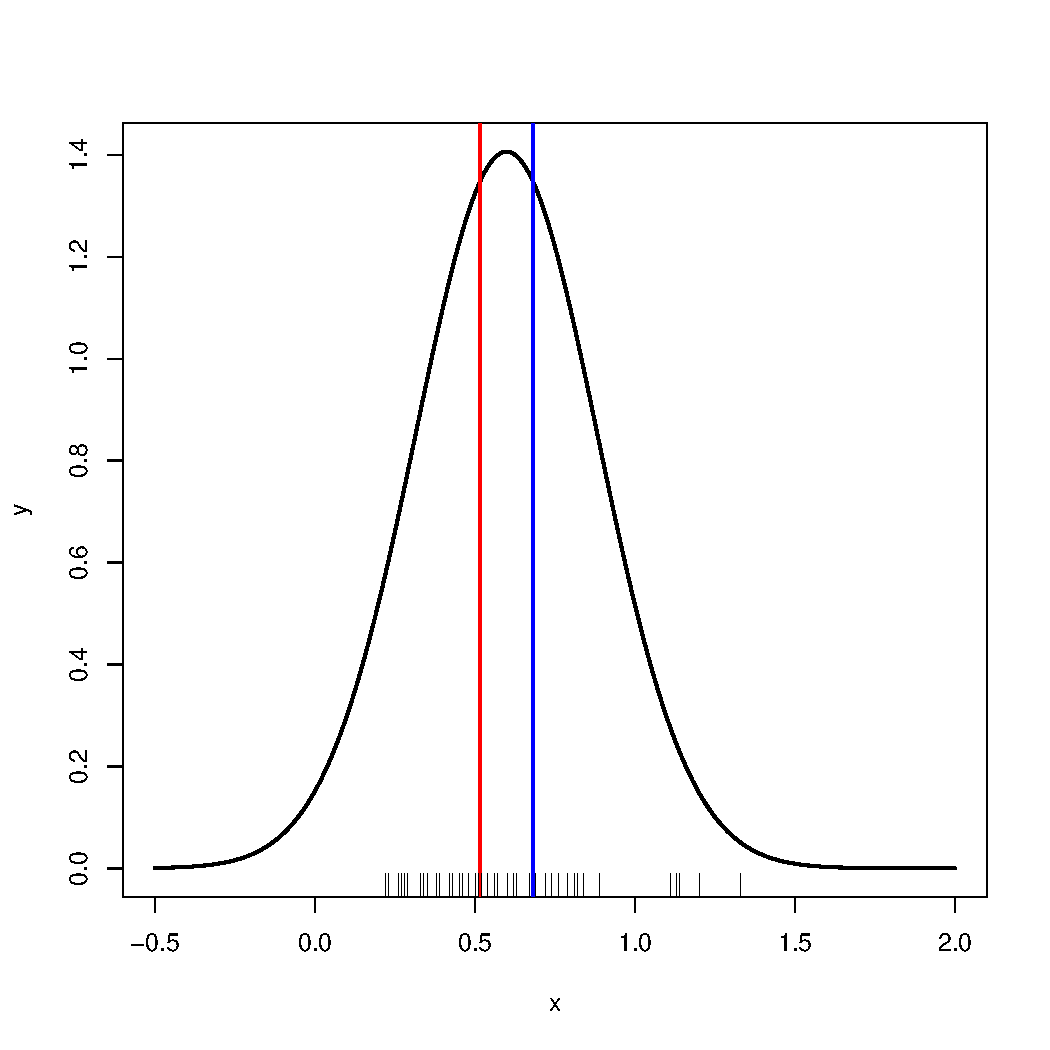
\includegraphics[width=\maxwidth]{figure/parmetricfigure-1} 

\end{knitrout}

\end{marginfigure}

\section{Is the value outside the expected range?}

When our sample size is small relative to the population size, we can use the following formula to calculate a z-value, 

\begin{equation}
z = \frac{\bar{y}-\mu}{\sigma/\sqrt{n}}
\end{equation}

z follows a z-distribution or a standard normal distribution ($z\sim(0,1)$), thus can be used to evaluate probilities.  

With our ten numbers, we can then compare z to the standard normal distribution, 





\subsection{Distribution Free Confidence Intervals}

The simplest way to calculate a distribution-free confidence interval is to simply calculate the percentile of the data. However, rarely do we have enough data to have these percentages represented. So, what can we do?

In progress...

\subsection{Bootstrapping Confidence Intervals}

Similar to the distribution-free methods, the bootstrapping method creates confidence intervals based on the data themselves without the use of a theoretical distribution. In this case, we ''sample'' our dataset over and over again to create a distribution of t-values from which to create confidence intervals. 

Let's begin to sampling the copper data. First, we want to sample the data (with replacement) to create a sample. 

\begin{knitrout}
\definecolor{shadecolor}{rgb}{0.969, 0.969, 0.969}\color{fgcolor}\begin{kframe}
\begin{alltt}
\hlkwd{sample}\hlstd{(TcCB_ref,} \hlkwd{length}\hlstd{(TcCB_ref),} \hlkwc{replace}\hlstd{=T)}
\end{alltt}
\begin{verbatim}
##  [1] 0.29 0.23 0.76 1.14 0.63 1.11 0.69 0.51 0.39 0.67 0.46
## [12] 0.57 0.28 1.13 1.11 0.27 1.14 0.56 0.67 0.35 0.74 1.14
## [23] 0.76 0.38 0.28 1.14 0.39 1.13 1.11 0.82 0.48 0.39 0.48
## [34] 0.89 0.42 0.67 1.14 0.69 0.42 0.76 0.39 0.27 0.26 0.50
## [45] 1.20 1.14 1.33
\end{verbatim}
\end{kframe}
\end{knitrout}

We'll call it sample.bs (bs = bootstrapped)

\begin{knitrout}
\definecolor{shadecolor}{rgb}{0.969, 0.969, 0.969}\color{fgcolor}\begin{kframe}
\begin{alltt}
\hlstd{sample.bs} \hlkwb{<-} \hlkwd{sample}\hlstd{(TcCB_ref,} \hlkwd{length}\hlstd{(TcCB_ref),} \hlkwc{replace}\hlstd{=T)}
\end{alltt}
\end{kframe}
\end{knitrout}

From this, we can create a t-value using the following formula

\begin{equation}
t = (\bar{x} - \mu)/(s/sqrt{n})
\end{equation}

where $\mu$ is the population mean, 0.5985106, calculated from the original dataset. 

\begin{knitrout}
\definecolor{shadecolor}{rgb}{0.969, 0.969, 0.969}\color{fgcolor}\begin{kframe}
\begin{alltt}
\hlstd{mean.bs} \hlkwb{<-} \hlkwd{mean}\hlstd{(sample.bs);}
\hlstd{sd.bs} \hlkwb{<-} \hlkwd{sd}\hlstd{(sample.bs);}
\hlstd{n.bs} \hlkwb{<-} \hlkwd{length}\hlstd{(sample.bs)}
\hlstd{t} \hlkwb{=} \hlstd{(mean.bs} \hlopt{-} \hlstd{TcCB_ref_mean)}\hlopt{/}\hlstd{(sd.bs}\hlopt{/}\hlkwd{sqrt}\hlstd{(n.bs)); t}
\end{alltt}
\begin{verbatim}
## [1] 0.868128
\end{verbatim}
\end{kframe}
\end{knitrout}

And now, we want to do this lots of time to create a distribution of $t_i$ that we can find the bottom 0.025\% and top 0.975\%. 

First, let's create a loop to iterate 20 times.\sidenote{Notice that I complicated the t calculation by putting in the mean, sd, and length functions within the formula.}

\begin{knitrout}
\definecolor{shadecolor}{rgb}{0.969, 0.969, 0.969}\color{fgcolor}\begin{kframe}
\begin{alltt}
\hlstd{t} \hlkwb{<-} \hlkwd{vector}\hlstd{()}
\hlstd{iterations} \hlkwb{=} \hlnum{20}
\hlkwd{set.seed}\hlstd{(}\hlnum{666}\hlstd{)}
\hlkwa{for}\hlstd{(i} \hlkwa{in} \hlnum{1}\hlopt{:}\hlstd{iterations)\{}
  \hlstd{sample.bs} \hlkwb{<-} \hlkwd{sample}\hlstd{(}\hlkwc{x}\hlstd{=TcCB_ref,} \hlkwc{size}\hlstd{=}\hlkwd{length}\hlstd{(TcCB_ref),} \hlkwc{replace}\hlstd{=T)}
  \hlstd{t[i]} \hlkwb{<-} \hlstd{(}\hlkwd{mean}\hlstd{(sample.bs)} \hlopt{-} \hlstd{TcCB_ref_mean)}\hlopt{/}\hlstd{(}\hlkwd{sd}\hlstd{(sample.bs)}\hlopt{/}\hlkwd{sqrt}\hlstd{(}\hlkwd{length}\hlstd{(sample.bs)))}
\hlstd{\}}
\end{alltt}
\end{kframe}
\end{knitrout}

Note that with 20 samples how ''bumpy'' the line looks (Figure \ref{fig:t20}). In fact, it appears to look nothing like the t-Distribution. Let's increase the number of iterations to 5000 and see what happens next.

\begin{marginfigure}
\begin{knitrout}
\definecolor{shadecolor}{rgb}{0.969, 0.969, 0.969}\color{fgcolor}
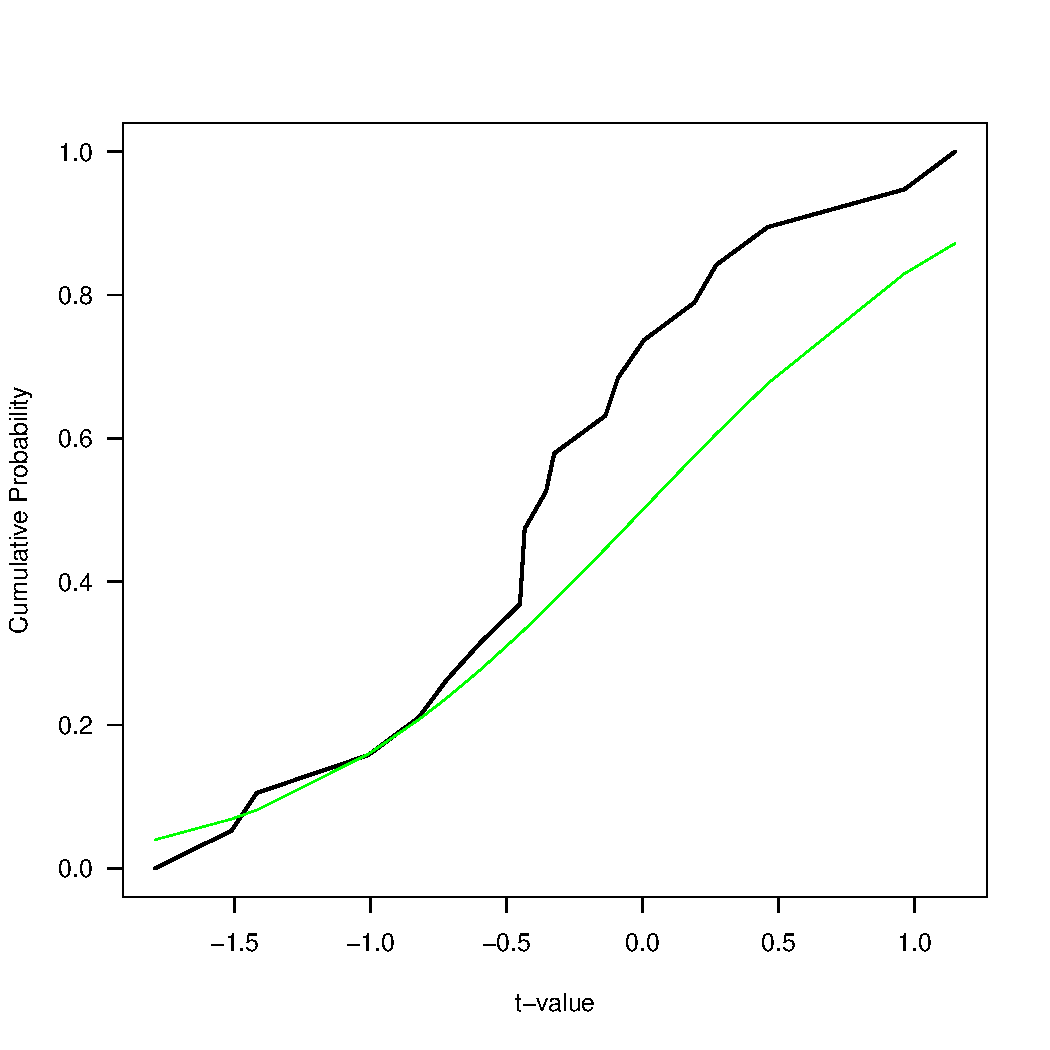
\includegraphics[width=\maxwidth]{figure/cdf_20-1} 

\end{knitrout}
	\caption{t-values with 20 interactions}
	\label{fig:t20}
\end{marginfigure}





So, let's look at a histogram of the t-values we bootstrapped (Table \ref{fig:hist-bs}). Notice that the distribution approximates a normal distribution. In spite of this, the confidence intervals using this method will vary.


\begin{marginfigure}
\begin{knitrout}
\definecolor{shadecolor}{rgb}{0.969, 0.969, 0.969}\color{fgcolor}
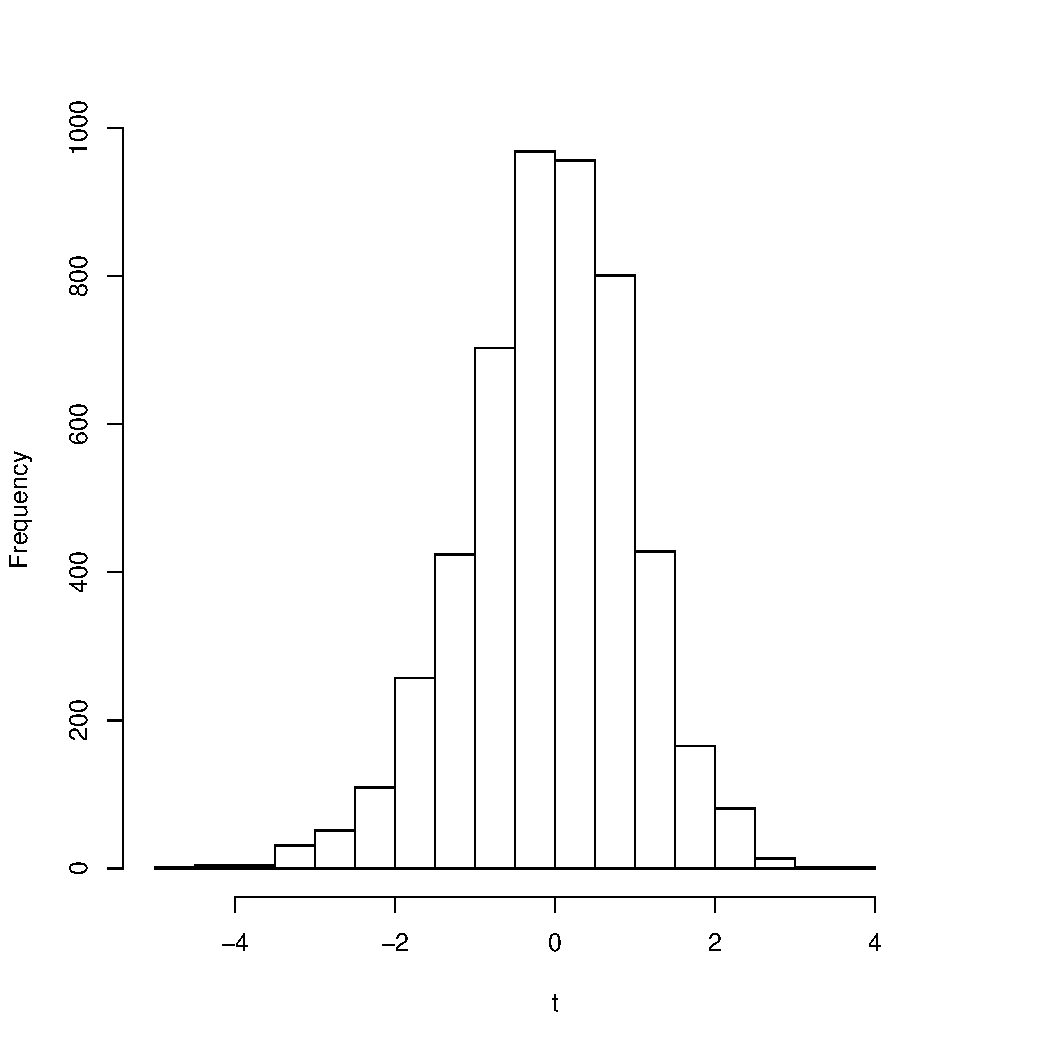
\includegraphics[width=\maxwidth]{figure/histbs-1} 

\end{knitrout}
	\caption{Histogram of 5,000 bootstrapped t-values.}
	\label{fig:hist-bs}
\end{marginfigure}

Now, let's create a cumulative distribution of our t-values. First, we put them in order and create a sequence of probabilities for each t-value (each one is equally probable, so this is pretty easy. We create a sequence of probabilities, y, that is the same number of interactions.

\begin{knitrout}
\definecolor{shadecolor}{rgb}{0.969, 0.969, 0.969}\color{fgcolor}\begin{kframe}
\begin{alltt}
\hlstd{t} \hlkwb{<-} \hlkwd{sort}\hlstd{(t)}
\hlstd{y} \hlkwb{<-} \hlkwd{seq}\hlstd{(}\hlnum{0}\hlstd{,} \hlnum{1}\hlstd{,} \hlkwc{length.out} \hlstd{= iterations)}
\end{alltt}
\end{kframe}
\end{knitrout}


\begin{figure}
\begin{knitrout}
\definecolor{shadecolor}{rgb}{0.969, 0.969, 0.969}\color{fgcolor}
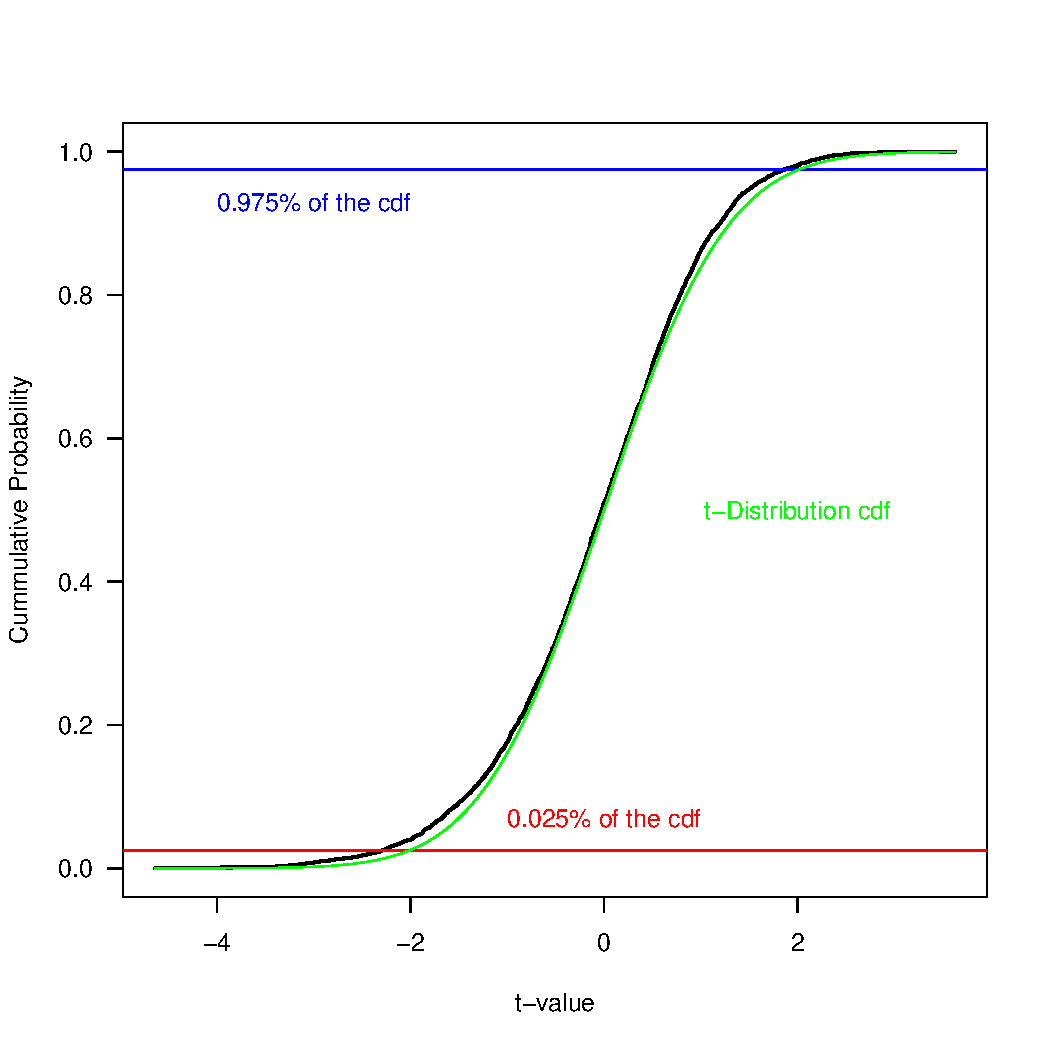
\includegraphics[width=\maxwidth]{figure/cdf_5000-1} 

\end{knitrout}
	\caption{Cumlative with CIs}
	\label{CumCI}
\end{figure}

So, finally, we can query the t-values themselves to find the 0.025\% and 0.975\% percentiles. 

\begin{knitrout}
\definecolor{shadecolor}{rgb}{0.969, 0.969, 0.969}\color{fgcolor}\begin{kframe}
\begin{alltt}
\hlstd{t.low}  \hlkwb{<-} \hlstd{t[}\hlnum{0.025} \hlopt{*} \hlstd{iterations]}
\hlstd{t.high} \hlkwb{<-} \hlstd{t[}\hlnum{0.975} \hlopt{*} \hlstd{iterations]}
\end{alltt}
\end{kframe}
\end{knitrout}

Then we plug these into the following formula to get the confidence intervals

\begin{equation}
\bar{x} - t_{high}(s/\sqrt{n}) < \mu < \bar{x} - t_{low}(s/\sqrt{n}) 
\end{equation}



And I get 0.522 $ < \mu < $ 0.693. 

% Calculate values for clean up site.



Your answer may vary if you did not set the seed the same as I did. These are fairly close to the parametric estimates. Because these data are fairly well behaved, we didn't see a big difference, but when you do the same analysis with the cleaned up site the results are quite different. For the parametric results, the confidence intervals are -0.611 and 8.534 and for the bootstrapped values, 0.846 and 58.56. 




% Book example -- but I didn't get the same results, but Manly may not have extrapolated carefully?

\begin{knitrout}
\definecolor{shadecolor}{rgb}{0.969, 0.969, 0.969}\color{fgcolor}
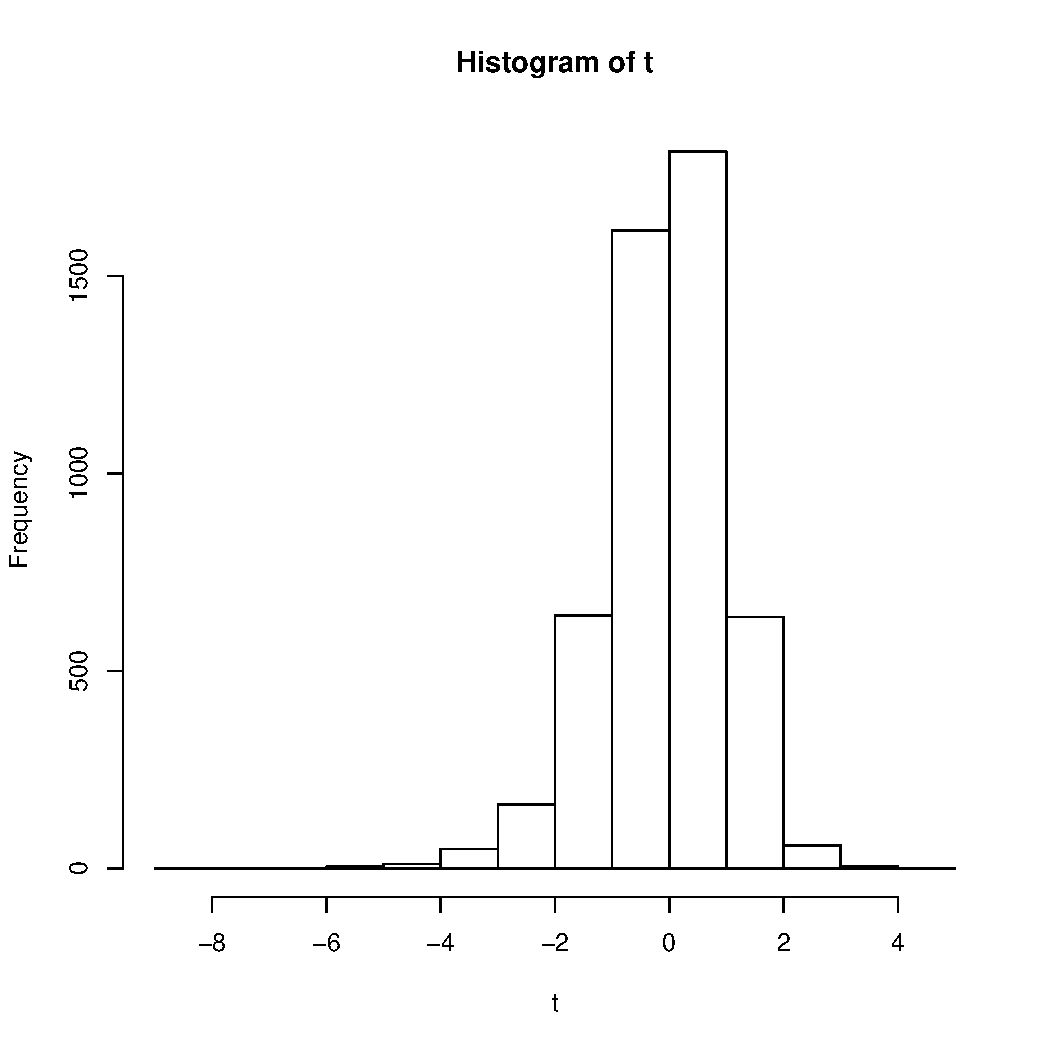
\includegraphics[width=\maxwidth]{figure/bookexample-1} 

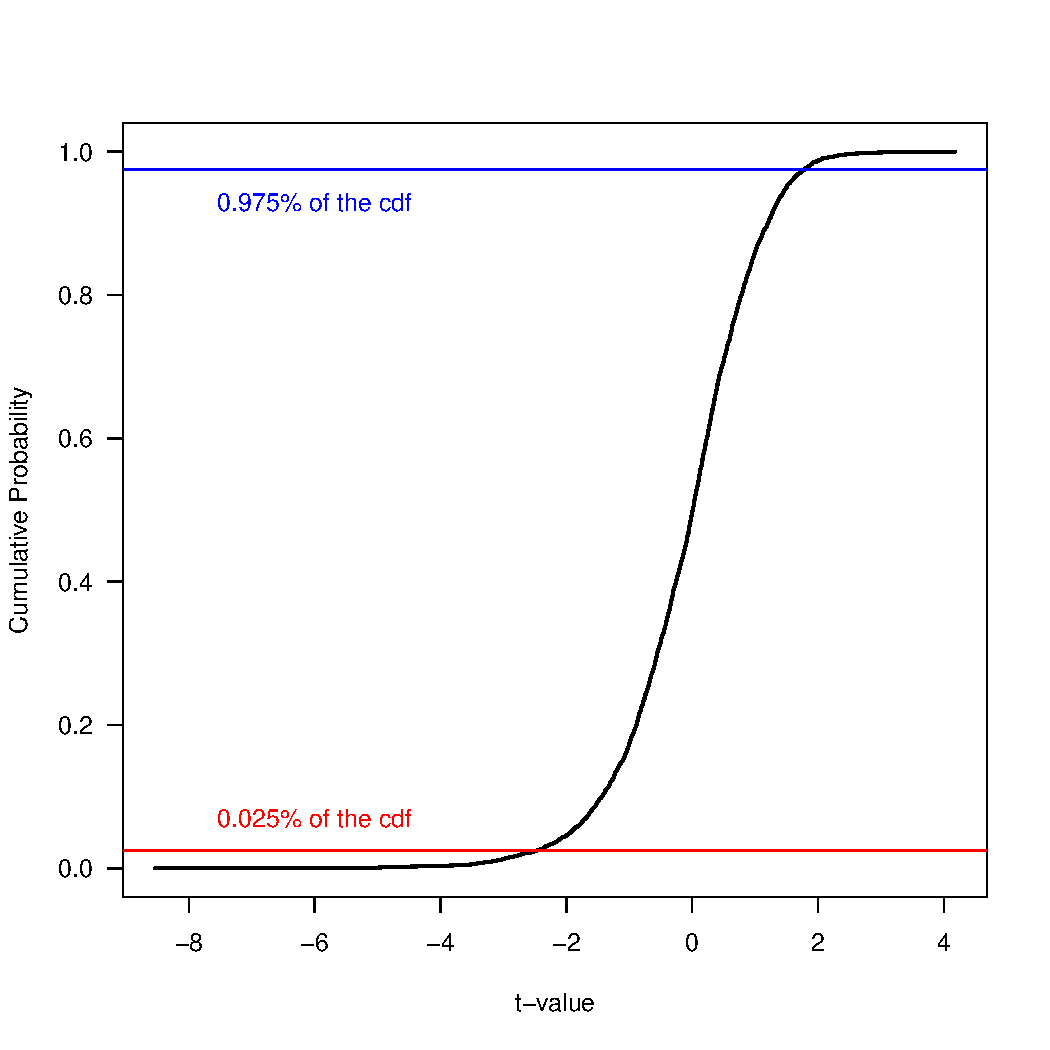
\includegraphics[width=\maxwidth]{figure/bookexample-2} 

\end{knitrout}



\subsection{Maximum Likelihood Methods}

To be developed!


\subsection{Bayesian Confidence Intervals}

To be developed!

Confidence intervals are one method of interval estimation, and the most widely used in frequentist statistics. An analogous concept in Bayesian statistics is credible intervals, while an alternative frequentist method is prediction interval, which, rather than estimating parameters, estimates the outcome of future samples.

There is disagreement about which of these methods produces the most useful results: the mathematics of the computations are rarely in question Ö confidence intervals being based on sampling distributions, credible intervals being based on Bayes' theorem Ö but the application of these methods, the utility and interpretation of the produced statistics, is debated.

Users of Bayesian methods, if they produced an interval estimate, would in contrast to confidence intervals, want to say "My degree of belief that the parameter is in fact in this interval is 90\%," while users of prediction intervals would instead say "I predict that the next sample will fall in this interval 90\% of the time."

Confidence intervals are an expression of probability and are subject to the normal laws of probability. If several statistics are presented with confidence intervals, each calculated separately on the assumption of independence, that assumption must be honored or the calculations will be rendered invalid. For example, if the statistic with the narrowest interval were selected for attention, that interval would no longer be the true interval for that statistic. The act of selection changes the probability and in this case widens the interval.

This is particularly important when confidence intervals are generated in order to perform statistical tests. If multiple tests are done and those that return positive results are selected from amongst them, the intervals used to conduct the test will change, and in most situations the tests will be rendered invalid.

A Bayesian interval estimate is called a credible interval. Using much of the same notation as above, the definition of a credible interval for the unknown true value of ? is, for a given ?[4],

  $  \Pr(u(x)<\Theta<v(x) | X = x)=1-\alpha. \, $

Here ? is used to emphasize that the unknown value of ? is being treated as a random variable. The definitions of the two types of intervals may be compared as follows.

    * The definition of a confidence interval involves probabilities calculated from the distribution of X for given (?, ?) (or conditional on these values) and the condition needs to hold for all values of (?, ?).
    * The definition of a credible interval involves probabilities calculated from the distribution of ? conditional on the observed values of X = x and marginalised (or averaged) over the values of ?, where this last quantity is the random variable corresponding to the uncertainty about the nuisance parameters in ?.

Note that the treatment of the nuisance parameters above is often omitted from discussions comparing confidence and credible intervals but it is markedly different between the two cases.

In some simple standard cases, the intervals produced as confidence and credible intervals from the same data set can be identical. They are always very different if moderate or strong prior information is included in the Bayesian analysis.



\section{Confidence Intervals Applied to Accuracy}

To be developed!

Accuracy is also used as a statistical measure of how well a binary classification test correctly identifies or excludes a condition. This can be explicitly categorized in determine detection limits (Table \ref{tab:HypothesisTesting}).

\begin{table}
	\centering
		\begin{tabular}{l |l | l | l | l}
&&True Condition&& \\
&& True & False & \\
Test Outcome& Positive & True Positive & False Positive & Positive predictive value \\
Test Outcome& Negative & False Positive & True Negative & Negative predictive value \\
&& Sensitivity & Specificity & Accuracy	
		\end{tabular}
	\caption{Hypothesis Testing}
	\label{tab:HypothesisTesting}
\end{table}


That is, the accuracy is the proportion of true results (both true positives and true negatives) in the population. It is a parameter of the test.

\begin{equation}
accuracy=\frac{\text{number of true positives}+\text{number of true negatives}}{\text{numbers of true positives}+\text{false positives} + \text{false negatives} + \text{true negatives}}
\end{equation}

On the other hand, precision is defined as the proportion of the true positives against all the positive results (both true positives and false positives)

\begin{equation}
precision=\frac{\text{number of true positives}}{\text{number of true positives}+\text{false positives}}
\end{equation}

An accuracy of 100\% means that the measured values are exactly the same as the given values.

Also see Sensitivity and specificity.

Accuracy may be determined from Sensitivity and Specificity, provided Prevalence is known, using the equation:

    accuracy = (sensitivity)(prevalence) + (specificity)(1 - prevalence)

The accuracy paradox for predictive analytics states that predictive models with a given level of accuracy may have greater predictive power than models with higher accuracy. It may be better to avoid the accuracy metric in favor of other metrics such as precision and recall.



\end{comment}

\FloatBarrier 
\begin{fullwidth}
% \renewcommand{\bibfont}{\small}
%\bibliography{LosHuertos_Complete_100420}
%\bibliographystyle{cbe}
\end{fullwidth}

\end{document}
